%\documentclass[CJK]{beamer}  


\usepackage{fontspec,xunicode,xltxtra,beamerthemesplit,listings}

\usepackage[caption=false,font=footnotesize]{subfig}
\usepackage{tikz}
\usetikzlibrary{shapes,arrows,shadows,mindmap,backgrounds}

\usetheme{Warsaw} 
\useoutertheme{infolines}

\setbeamercovered{transparent}
\setbeamertemplate{items}[circle]
\renewcommand{\figurename}{図}
\newtheorem{definationfc}{定義}

\usepackage[overlap,CJK]{ruby}
\usepackage{multicol}
%\usepackage[sort&compress]{natbib}
%\usepackage{chapterbib}

\newcommand{\backupbegin}{
   \newcounter{framenumberappendix}
   \setcounter{framenumberappendix}{\value{framenumber}}
}
\newcommand{\backupend}{
   \addtocounter{framenumberappendix}{-\value{framenumber}}
   \addtocounter{framenumber}{\value{framenumberappendix}} 
}



\setmainfont{MS PGothic}
\setsansfont{Meiryo UI} %[Mapping=tex-text]
\setmonofont{Courier New}


\def\beamer@linkspace#1{%
  \begin{pgfpicture}{0pt}{-1.5pt}{#1}{5.5pt}
    \pgfsetfillopacity{0}
    \pgftext[x=0pt,y=-1.5pt]{.}
    \pgftext[x=#1,y=5.5pt]{.}
  \end{pgfpicture}}

\lstset{tabsize=4, %
  frame=shadowbox, %把代码用带有阴影的框圈起来
  commentstyle=\color{red!50!green!50!blue!50},%浅灰色的注释
  rulesepcolor=\color{red!20!green!20!blue!20},%代码块边框为淡青色
  keywordstyle=\color{blue!90}\bfseries, %代码关键字的颜色为蓝色,粗体
  showstringspaces=false,%不显示代码字符串中间的空格标记
  stringstyle=\ttfamily, % 代码字符串的特殊格式
  keepspaces=true, %
  breakindent=22pt, %
  numbers=left,%左侧显示行号
  stepnumber=1,%
  numberstyle=\tiny, %行号字体用小号
  basicstyle=\footnotesize, %
  showspaces=false, %
  flexiblecolumns=true, %
  breaklines=true, %对过长的代码自动换行
  breakautoindent=true,%
  breakindent=4em, %
  aboveskip=1em, %代码块边框
  %% added by http://bbs.ctex.org/viewthread.php?tid=53451
  fontadjust,
  captionpos=t,
  framextopmargin=2pt,framexbottommargin=2pt,abovecaptionskip=-3pt,belowcaptionskip=3pt,
  xleftmargin=4em,xrightmargin=4em, % 设定listing左右的空白
  texcl=true,
  % 设定中文冲突,断行,列模式,数学环境输入,listing数字的样式
  extendedchars=false,columns=flexible,mathescape=true
  numbersep=-1em
}

%%%%%%%%%%%%%%%%%%%%%%%%%%%%%%%%%%%%%%%%%%%%%%%%%%%%%%%%%%%%%%%%%%%%%%%%

\title[チェックリストと分割に基づく網羅と使用テスト]{
チェックリストと分割に基づく 網羅と使用テスト\\
{\small\scshape Coverage and Usage Testing Based on Checklists and Partitions}}

\subtitle[B4M1 輪講]{第8章 ($p107\sim p126$) B4M1 輪講}

\author[大阪大学大学院CS専攻\quad{}楊 嘉晨]{修士課程1年生\quad{}楊 嘉晨}
\institute[楠本研]{大阪大学大学院 コンピュータサイエンス専攻 楠本研究室}
\date{2012年5月29日(火)}

\pgfdeclareimage[height=0.618cm]{logo}{figure/logo.pdf}
\logo{\pgfuseimage{logo}}

\mode<article>{\providecommand{\imageheight}{0.2\textheight}}
\mode<presentation>{\providecommand{\imageheight}{0.4\textheight}}

%%%%%%%%%%%%%%%%%%%%%%%%%%%%%%%%%%%%%%%%%%%%%%%%%%%%%%%%%%%%%%%%%%%%%%%%
\begin{document} 

\mode<presentation>{

\providecommand{\newblock}{\\}
\providecommand{\toprule}{\hline}
\providecommand{\midrule}{\hline}
\providecommand{\bottomrule}{\hline}
\providecommand{\itemtitle}[1]{\item \alert{#1} \quad{} }
}

\mode<article>{
\renewenvironment{columns}{\begin{multicols}{2}}{\end{multicols}\\}
\renewenvironment{column}[1]{}{}
}

\XeTeXlinebreaklocale "jp"  
\XeTeXlinebreakskip = 0pt plus 1pt 

\frame{\titlepage} 
\mode<article>{\maketitle}

\begin{frame}<trans|beamer>[shrink=10]{目次}
\tableofcontents[section,subsectionstyle=hide,subsubsectionstyle=hide] 
\end{frame}


\AtBeginSubsection[]{
  \begin{frame}<trans|beamer>[shrink=25]{目次}
    \tableofcontents[sectionstyle=show/shaded,subsectionstyle=show/shaded/hide] 
  \end{frame}
}

%%%%%%%%%%%%%%%%%%%%%%%%%%%%%%%%%%%%%%%%%%%%%%%%%%%%%%%%%%%%%%%%%%%%%%%%
\section{第8章の概要}
\subsection{概要}
\begin{frame}{概要(p103)}

%\transwipe[direction=-90]

チェックリストや分割(Partition)等簡単なモデルで正規テストの手法について紹介

\begin{enumerate}
\item 8.1節, 様々なチェックリストで正規と半正規のテスト
\item 8.2節, チェックリストを分割に正規化して, 簡単なカバレッジテストを行い
\item 8.3節, 操作プロフィール(Operation Profile, OP)という,
    分割のために簡単なUBT(Usage-based Testing)を紹介
\item 8.4節, OPを生成する手順
\item 8.5節, Case Study
\end{enumerate}

第9章には, 分割した入力サブドメインの境界条件のテストについて, 似ているモデルを紹介

\end{frame}
%%%%%%%%%%%%%%%%%%%%%%%%%%%%%%%%%%%%%%%%%%%%%%%%%%%%%%%%%%%%%%%%%%%%%%%%

\section{8.1 チェックリストに基づくテスト, とその制限}
\subsection{チェックリストに基づくテスト(Testing with Checklists)}

\begin{frame}{Ad hocテスト と ランダムテスト(p104)}
\framesubtitle{Ad hoc Testing \& Random Testing}


\pgfdeclareimage[height=\imageheight]{Ad-Hoc-Testing}{figure/Ad-Hoc-Testing.jpg}
\pgfdeclareimage[height=\imageheight]{Random-Testing}{figure/Random-Testing.jpg}

\transwipe[direction=0]<2>
\transwipe[direction=180]<3>

%\mode<presentation>{
\begin{columns}[t]
\begin{column}{.5\textwidth}
\only<1,3>{
\begin{figure}
\begin{center}
\pgfuseimage{Ad-Hoc-Testing}
\caption{Ad hot Testing}
\end{center}
\end{figure}

}

\end{column}
\begin{column}{.5\textwidth}
\only<2,3>{
\begin{figure}
\begin{center}
\pgfuseimage{Random-Testing}
\caption{Random Testing}
\end{center}
\end{figure}
}
\end{column}
\end{columns}

\begin{overprint}
\onslide<1|handout:0|trans:0|article:0> ソフトウェアを\alert{勝手に}実行してその結果を観察
\onslide<2|handout:0|trans:0|article:0>
\alert{統計的}にランダムのプロフィールでテストの操作を行う
\onslide<3|handout:1|trans:1|article:1> 繰り返してAd hocテストを実行する時,
    テスト者は行ったテストを追跡すると, チェックリストテストになる
\end{overprint}
%}

%\mode<article>{
%図~\ref{fig:adhoc}ソフトウェアを\alert{勝手に}実行してその結果を観察
%
%図~\ref{fig:random} \alert{統計的}にランダムのプロフィールでテストの操作を行い
%
%繰り返してAd hocテストを実行する時, 試験者は行ったテストを追跡すると, チェックリストテストになった
%
%\begin{figure}
%\begin{center}
%\label{fig:adhoc}
%\pgfuseimage{Ad-Hoc-Testing}
%\caption{Ad Hot Testing}
%\end{center}
%\end{figure}
%\begin{figure}
%\begin{center}
%\label{fig:random}
%\pgfuseimage{Random-Testing}
%\caption{Random Testing}
%\end{center}
%\end{figure}
%}

\end{frame}

%%%%%%%%%%%%%%%%%%%%%%%%%%%%%%%%%%%%%%%%%%%%%%%%%%%%%%%%%%%%%%%%%%%%%%%%

\begin{frame}[shrink=15]{チェックリストに基づくテスト(p104)}
\framesubtitle{Testing with checklists}
\transfade<2>[duration=0.5]
\mode<article>{\renewcommand{\imageheight}{0.2\textheight}}
\mode<presentation>{\renewcommand{\imageheight}{0.5\textheight}}
\pgfdeclareimage[height=\imageheight]{checklist}{figure/checklist.jpg}
\pgfdeclareimage[height=\imageheight]{blackboxchecklist}{figure/blackboxchecklist.png}
\begin{columns}[t]
    \begin{column}{.6\textwidth}
    \begin{itemize}
    \item ブラックボックステスト(BBT)
        \begin{itemize}
        \item ソフトウェア要求チェックリスト
        \item 機能チェックリスト
            \begin{itemize}
            \item システム全体からハイレベルの機能
            \item ローレベルの字句, 独立な部品
            \end{itemize}
        \end{itemize}
    \item ホワイトボックステスト(WBT)
        \begin{itemize}
        \item プログラムの特徴
        \item コーディング標準
        \item 単体テストの文の網羅
        \item 統合テストとシステムテストの部品の網羅
        \item 構造と特徴など, 実装に関しるチェックリスト
            \begin{itemize}
            \item 関数の呼び出し規則
            \item 資源の生産者と消費者
            \item モジュール間に共有するデータ
            \end{itemize}
        \end{itemize}
    \end{itemize}
    \end{column}
        \begin{column}{.35\textwidth}
        \begin{figure}
        \begin{center}
            \begin{overlayarea}{\textwidth}{0.6\textheight}
            \begin{center}
            \only<1|handout:0|trans:0|article:0>{\pgfuseimage{checklist}}
            \only<2|handout:1|trans:1>{\pgfuseimage{blackboxchecklist}}
            \end{center}
            \end{overlayarea}
        \caption{チェックリスト}
        \end{center}
        \end{figure}
    \end{column}
\end{columns}
\end{frame}
%%%%%%%%%%%%%%%%%%%%%%%%%%%%%%%%%%%%%%%%%%%%%%%%%%%%%%%%%%%%%%%%%%%%%%%%
\subsection{階層及び複合チェックリスト(Hierarchical and Combined Checklists)}
\begin{frame}{階層チェックリスト(p105)}
\framesubtitle{Hierarchical Checklists }
\begin{columns}
    \begin{column}{0.35\textwidth}
    \flushright{
    \begin{enumerate}
    \item ハイレベル項目1
    \item ハイレベル項目2
    \item ハイレベル項目3
    \end{enumerate}
    }
    \end{column}
    \begin{column}{0.05\textwidth}
    \Huge\[\Rightarrow\]
    \end{column}
    \begin{column}{0.5\textwidth}
    \begin{enumerate}
    \item ハイレベル項目1
        \begin{enumerate}
        \item ローレベル項目1
        \item ローレベル項目2
        \item ローレベル項目3
        \end{enumerate}
    \item ハイレベル項目2
        \begin{enumerate}
        \item ローレベル項目4
        \item ローレベル項目5
        \end{enumerate}
    \item ハイレベル項目3
        \begin{enumerate}
        \item ローレベル項目6
        \item ローレベル項目7
        \item ローレベル項目8
        \end{enumerate}
    \end{enumerate}
    \end{column}
\end{columns}
\end{frame}
%%%%%%%%%%%%%%%%%%%%%%%%%%%%%%%%%%%%%%%%%%%%%%%%%%%%%%%%%%%%%%%%%%%%%%%%
\begin{frame}[shrink=5]{複合チェックリスト(p105)}
\framesubtitle{Combined Checklists}
\pgfdeclareimage[height=\imageheight]{2dchecklist}{figure/2dchecklist.png}
\transfade<2->[duration=0.5]

\begin{tabular}{lc}
& \begin{actionenv}<uncover@3|alert@3|article:0> 要求1 \quad 要求2 \quad 要求3\end{actionenv} \\
\begin{minipage}{0.3\textwidth}
\begin{enumerate}
\begin{actionenv}<uncover@1-3>
\item 部品1
    \begin{actionenv}<uncover@2,3 | alert@3>
    \begin{enumerate}
    \item 要求1
    \item 要求2
    \item 要求3
    \end{enumerate}
    \end{actionenv}
\item 部品2
    \begin{actionenv}<uncover@2,3 | alert@3>
    \begin{enumerate}
    \item 要求1
    \item 要求2
    \item 要求3
    \end{enumerate}
    \end{actionenv}
\item 部品3
    \begin{actionenv}<uncover@2,3 | alert@3>
    \begin{enumerate}
    \item 要求1
    \item 要求2
    \item 要求3
    \end{enumerate}
    \end{actionenv}
\end{actionenv}
\end{enumerate} 
\end{minipage} & 
\mode<presentation>{\visible<4>{
    \begin{minipage}{0.4\textwidth}
        \begin{figure}
            \begin{center}
            \pgfuseimage{2dchecklist}
            \end{center}
        \caption{標準チェックリストと部品チェックリストを複合した二次元表}
        \end{figure}
    \end{minipage}
}}
\end{tabular}

\mode<article>{
\begin{figure}
    \begin{center}
    \pgfuseimage{2dchecklist}
    \end{center}
\caption{標準チェックリストと部品チェックリストを複合した二次元表}
\end{figure}
}
\end{frame}

%%%%%%%%%%%%%%%%%%%%%%%%%%%%%%%%%%%%%%%%%%%%%%%%%%%%%%%%%%%%%%%%%%%%%%%%
\subsection{チェックリストの問題点と制限(Problems and Limits of Checklists)}
\begin{frame}{チェックリストの問題点(p106)}
\framesubtitle{Problems General Checklists}

\begin{itemize}
\item チェックリストの定義が抽象的過ぎて, 具体的にするのが難しい
    \begin{itemize}
    \item 特にハイレベル
    \end{itemize}
\item 具体的なテストケースに変換するのは
    \begin{itemize}
    \item 経験が必要
    \item 特殊な環境や設定等に依存
    \end{itemize}
\item 大規模で, 複雑なシステムに, 相互接続と相互作用を定義するのも難しい 
    \note[item]{相互接続:そうごせつぞく}
    \note[item]{相互作用:そうごさよう}
\end{itemize}

\end{frame}
%%%%%%%%%%%%%%%%%%%%%%%%%%%%%%%%%%%%%%%%%%%%%%%%%%%%%%%%%%%%%%%%%%%%%%%%
\begin{frame}{チェックリストの制限(p106)}
\framesubtitle{Limitations of General Checklists}
\transfade<2->[duration=0.5]
\begin{enumerate}
\item 全部の機能(ブラックボックステスト)又は構造部品
(ホワイトボックステスト)を, 異なる視点や保証レベルから, 
網羅することが難しい
    \begin{itemize}
    \item 網羅されていない穴(Hole)が残ってしまう
    \item<uncover@3-|alert@3> 分割したチェックリストを使う
    \end{itemize}
\item より高い網羅率を目標にすると, テストを重複でしまう
    \begin{itemize}
    \item 無駄なテストを行われてしまう
    \item<uncover@3-|alert@3> 分割したチェックリストを使う
    \end{itemize}
\item 各システムの部品間の複雑な相互作用を定義するのは難しい
    \begin{itemize}
    \item<uncover@2-|alert@2> 10, 11章にFSMに基づく体系的な正規モデルを紹介
    \note[item]{体系的:たいけいてき} \note[item]{FSM: 有限状態機械(ゆうげんじょうたいきかい), 有限オートマトン}
    \end{itemize}
\end{enumerate}
\end{frame}
%%%%%%%%%%%%%%%%%%%%%%%%%%%%%%%%%%%%%%%%%%%%%%%%%%%%%%%%%%%%%%%%%%%%%%%%
\section{8.2 分割カバレッジテスト(Testing for Partition Coverage)}
\subsection{紹介}
\begin{frame}{分割カバレッジテスト(p107)}
\framesubtitle{Testing for Partition Coverage}
\begin{itemize}
\item 分割を基づくテストは一種のチェックリスト・テスト
\item 分割は集合全体を徹底的に覆う \note[item]{覆う:おおう} \note[item]{徹底的:てっていてき}
    \begin{itemize}
    \item より高い\alert{網羅率}
    \end{itemize}
\item 分割はお互いに重複することができない
    \begin{itemize}
    \item より高い\alert{効率}
    \end{itemize}
\end{itemize}
\end{frame}
%%%%%%%%%%%%%%%%%%%%%%%%%%%%%%%%%%%%%%%%%%%%%%%%%%%%%%%%%%%%%%%%%%%%%%%%
\subsection{8.2.1 動機の事例(Some Motivational Examples)}
\begin{frame}{動機の事例(p107)}
\framesubtitle{Some Motivational Examples}
\mode<article>{\renewcommand{\imageheight}{0.15\textheight}}
\mode<presentation>{\renewcommand{\imageheight}{0.35\textheight}}
%\transfade<2->[duration=0.5]
\begin{columns}
\begin{column}{0.5\textwidth}
\[ ax^2+bx+c = 0 \]
\pause
その解を求めると
\[ r=\frac{-b \pm \sqrt{b^2-4ac}}{2a} \]
\pause
全部可能な入力の組み合わせ
\[ 2^{32} \times 2^{32} \times 2^{32} = 2^{96}\]
\end{column}
\begin{column}{0.5\textwidth}
\only<4->{
\pgfdeclareimage[height=\imageheight]{axbxc}{figure/axbxc.png}
\begin{figure}
\begin{center}
\pgfuseimage{axbxc}
\caption{$ax^2+bx+c=0$のテストケース}
\end{center}
\end{figure}
}
\end{column}
\end{columns}
\end{frame}
%%%%%%%%%%%%%%%%%%%%%%%%%%%%%%%%%%%%%%%%%%%%%%%%%%%%%%%%%%%%%%%%%%%%%%%%
\subsection{8.2.2 分割:概念と定義(Partition: Concepts and Definitions)}
\begin{frame}[shrink=10]{分割:概念と定義(p108)}
\framesubtitle{Partition: Concepts and Definitions}
\begin{columns}
\begin{column}{0.5\textwidth}
\begin{enumerate}
\item 分割した集合は相互に排他的
\note[item]{要素が2つの集合に共有されていることがない}
    \[ \forall i,j,i\neq j \Rightarrow G_i \cap G_j = \emptyset \]
\pause
\item 分割した集合の和集合は全体の集合
\note[item]{和集合に分割する前に元の集合の全てが含まれている}
    \[ \bigcup_{i=1}^{n} G_i = S \]
\end{enumerate}

\end{column}
\pause
\begin{column}{0.5\textwidth}
分割した集合は同値類になる
\begin{block}{対称律(symmetric)} $R(a,b) \Rightarrow R(b,a) $ \end{block}
\begin{block}{推移律(transitive)} $R(a,b) \wedge R(b,c) \Rightarrow R(a,c)$ \end{block}
\begin{block}{反射律(reflexive)} $R(a,a)$ が常に成り立つ \end{block}
\end{column}
\end{columns}
\end{frame}
%%%%%%%%%%%%%%%%%%%%%%%%%%%%%%%%%%%%%%%%%%%%%%%%%%%%%%%%%%%%%%%%%%%%%%%%
\subsection{8.2.3 分割テストの決定と網羅範囲の予測}
\begin{frame}{分割テストの網羅範囲の決定(p109)}
\framesubtitle{Testing Decisions for Partition Coverage}
分割テストは一種のチェックリストであり, 分割の種類は8.1節に
述べたチェックリストの種類に似ている. 
但し, 分割の決定は以下のとおりに決められている
\begin{enumerate}
\item 製品によって分割
    \begin{itemize}
    \item 例えば外部関数(BBT視点)又はシステム部品(WBT視点)
    \item<uncover@2-|alert@2>
    チェックリストと同じ
    \end{itemize}
\item 性質, 関係, 論理的な条件によって分割, 更に2つに分かれている
    \begin{itemize}
    \item 論理変数を論理演算子に繋がれる論理述語による \note[item]{述語:じゅつご}
    \item 数的な変数を比較演算子によって比較する
    \item<uncover@3-|alert@3>
    論理述語や比較演算によって入力区間を分割
    \item<uncover@4-|alert@4>
    決定木を使う
    \end{itemize}
\item 1と2の組み合わせ 
\end{enumerate}
\end{frame}
%%%%%%%%%%%%%%%%%%%%%%%%%%%%%%%%%%%%%%%%%%%%%%%%%%%%%%%%%%%%%%%%%%%%%%%%
\begin{frame}[fragile]{決定木によって分割(p110)}
\framesubtitle{Testing Decisions based on Decision Tree}
\transfade<2->[duration=0.5]

\begin{columns}
\begin{column}{0.5\textwidth}

\tikzstyle{level 1}=[level distance=1.5cm, sibling distance=2.5cm]
\tikzstyle{level 2}=[level distance=1cm, sibling distance=2cm]
\tikzstyle{level 3}=[level distance=1cm, sibling distance=1.5cm]
\tikzstyle{bag} = [rectangle, text width=6em, text centered, draw]
\tikzstyle{decision} = [rectangle, minimum height=8pt, minimum width=8pt, fill, inner sep=0pt]
\tikzstyle{choice} = [circle, minimum width=8pt, fill, inner sep=0pt]
\tikzstyle{end} = [regular polygon, regular polygon sides=3, minimum width=8pt, fill, inner sep=0pt,shape border rotate=90]

\begin{tikzpicture}[grow=right,child anchor=west]
\tiny
\node[bag]{\only<1|handout:0|trans:0|article:0>{最初決定}\only<2|handout:1|trans:1|article:1>{決定$P$}}
child {
    node[decision]{}
    child {
        node[bag]{\only<1|handout:0|trans:0|article:0>{中間決定1}\only<2|handout:1|trans:1|article:1>{決定$Q$}}
            child{
                node[choice]{}
                child {
                    node[bag]{\only<1|handout:0|trans:0|article:0>{結果1}\only<2|handout:1|trans:1|article:1>{$P \wedge Q$}}
                    child {
                        node[end]{}
                    }
                }
                child {
                    node[bag]{\only<1|handout:0|trans:0|article:0>{結果2}\only<2|handout:1|trans:1|article:1>{$P \wedge \neg Q$}}
                    child {
                        node[end]{}
                    }
                }
            }
    }
    child {
        node[bag]{\only<1|handout:0|trans:0|article:0>{中間決定2}\only<2|handout:1|trans:1|article:1>{決定$Q$}}
            child{
                node[choice]{}
                child {
                    node[bag]{\only<1|handout:0|trans:0|article:0>{結果3}\only<2|handout:1|trans:1|article:1>{$\neg P \wedge Q$}}
                    child {
                        node[end]{}
                    }
                }
                child {
                    node[bag]{\only<1|handout:0|trans:0|article:0>{結果4}\only<2|handout:1|trans:1|article:1>{$\neg P \wedge \neg Q$}}
                    child {
                        node[end]{}
                    }
                }
            }
        }
    };
\end{tikzpicture}

\only<1|handout:0|trans:0|article:0>{一貫性がない決定木}
\only<2|handout:1|trans:1|article:1>{一貫性を持つ決定木}

\uncover<2>{決定木によって, 一つの結果は一つの分割方法となって, パスを沿って結果を成り立たせる入力の範囲を求める}
\end{column}

\begin{column}{0.5\textwidth}
\begin{lstlisting}[language=java,escapechar=@]
if(@\only<1|handout:0|trans:0|article:0>{@最初決定@}\only<2|handout:1|trans:1|article:1>{@P@}@){
    if(@\only<1|handout:0|trans:0|article:0>{@中間決定1@}\only<2|handout:1|trans:1|article:1>{@Q@}@){
        @\only<1|handout:0|trans:0|article:0>{@結果1@}\only<2|handout:1|trans:1|article:1>{@$P \wedge Q$@}@;
    }else{
        @\only<1|handout:0|trans:0|article:0>{@結果2@}\only<2|handout:1|trans:1|article:1>{@$P \wedge \neg Q$@}@;
    }
}else{
    if(@\only<1|handout:0|trans:0|article:0>{@中間決定2@}\only<2|handout:1|trans:1|article:1>{@Q@}@){
        @\only<1|handout:0|trans:0|article:0>{@結果3@}\only<2|handout:1|trans:1|article:1>{@$\neg P \wedge Q$@}@;
    }else{
        @\only<1|handout:0|trans:0|article:0>{@結果4@}\only<2|handout:1|trans:1|article:1>{@$\neg P \wedge \neg Q$@}@;
    }
}
\end{lstlisting}
\end{column}
\end{columns}
\end{frame}
%%%%%%%%%%%%%%%%%%%%%%%%%%%%%%%%%%%%%%%%%%%%%%%%%%%%%%%%%%%%%%%%%%%%%%%%
\section{8.3 Musa氏の操作プロフィールで使用ベース統計的テスト}
\subsection{8.3.1 Usage-based統計的テストの場合}
\begin{frame}[shrink=13]{Usage-based統計的テスト適用場合(p111)}
\framesubtitle{The Cases for Usage-based Statistical Testing}
\transwipe<2->

\begin{columns}
\begin{column}{0.4\textwidth}
\begin{tabular}{lrl}
\hline
  操作   & \uncover<2->{頻度(\%)} & \\
\hline
スブドメイン1 &                      & \\
-操作1   & \uncover<2->{ 1\% }  & \\
-操作2   & \uncover<2->{72\% }  & \uncover<3->{$\checkmark$} \\
-操作3   & \uncover<2->{ 2\% }  & \\
スブドメイン2 &                      & \\
-操作4   & \uncover<2->{13\% }  & \uncover<3->{$\checkmark$} \\
-操作5   & \uncover<2->{ 2\% }  & \\
スブドメイン3 &                      & \\
-操作6   & \uncover<2->{ 3\% }  & \\
-操作7   & \uncover<2->{ 7\% }  & \uncover<3->{$\checkmark$} \\
\hline
\end{tabular}
\end{column}
\begin{column}{0.6\textwidth}
\only<4->{
\begin{enumerate}
\item 使用シナリオ, パターン, 関連する使用頻度を, ターゲットとなる消費者やユーザーから収集
\item 収集した情報を分析し, 操作プロフィール(OP, Operational Profile)に変換
\item 操作プロフィールによってテストを行い
\item テストの結果を分析し, 製品の信頼性を評価し, テストのフィードバックやソフトウェア開発プロセスに役立つ
    \begin{itemize}
    \item<uncover@5-> 製品の信頼性を評価する方法は22章に紹介する, 他のテストに関係する活動は7章に紹介した
    \end{itemize}
\end{enumerate}
}
\end{column}
\end{columns}
\end{frame}
%%%%%%%%%%%%%%%%%%%%%%%%%%%%%%%%%%%%%%%%%%%%%%%%%%%%%%%%%%%%%%%%%%%%%%%%
\begin{frame}{OPを開発プロセスに導入時期(p111)}
\framesubtitle{The Period of Development Process that Involves Operational Profiles}
\transfade<2->[duration=0.5]
\mode<article>{\renewcommand{\imageheight}{0.2\textheight}}
\mode<presentation>{\renewcommand{\imageheight}{0.7\textheight}}
\pgfdeclareimage[height=\imageheight]{vmodel}{figure/V-model.JPG}
\pgfdeclareimage[height=\imageheight]{vmodel-common}{figure/V-model-common.png}
\pgfdeclareimage[height=\imageheight]{vmodel-op}{figure/V-model-OP.png}
\begin{figure}
\begin{center}
\begin{overprint}
\onslide<1|handout:0|trans:0|article:0> \begin{center}\pgfuseimage{vmodel}\end{center}
\onslide<2|handout:0|trans:0|article:0> \begin{center}\pgfuseimage{vmodel-common}\end{center}
\onslide<3|handout:1|trans:1|article:1> \begin{center}\pgfuseimage{vmodel-op}\end{center}
\end{overprint}
\caption{操作プロフィールを開発プロセスに導入する時期}
\end{center}
\end{figure}
\end{frame}
%%%%%%%%%%%%%%%%%%%%%%%%%%%%%%%%%%%%%%%%%%%%%%%%%%%%%%%%%%%%%%%%%%%%%%%%
\subsection{8.3.2 Musa操作プロフィール:基本的な考え方(Musa OP:Basic Ideas)}
\begin{frame}[shrink=10]{MusaによるOPの定義(p112)}
\framesubtitle{Musa OP:Basic Ideas(Defination)}
\begin{definationfc}[操作プロフィール]
操作プロフィールとは, 一連の操作とそれらの出現
に関連する確率の配列 

An operational profile is a list of disjoint set of operations
and their associated probabilities of occurrence

\flushright{---\cite{musa1993operational}}
\end{definationfc}

\begin{thebibliography}{Musa(1993)}

\bibitem[Musa(1993)]{musa1993operational}
J.~Musa, ``Operational profiles in software-reliability engineering,''
  \emph{Software, IEEE}, vol.~10, no.~2, pp. 14--32, 1993.

\end{thebibliography}


\end{frame}

%%%%%%%%%%%%%%%%%%%%%%%%%%%%%%%%%%%%%%%%%%%%%%%%%%%%%%%%%%%%%%%%%%%%%%%%

\begin{frame}[shrink=10]{Musa OP:基本的な考え方(p113)}
\label{frame:basicideas}
\framesubtitle{Musa OP:Basic Ideas(Example)}
\mode<article>{\renewcommand{\imageheight}{0.2\textheight}}
\mode<presentation>{\renewcommand{\imageheight}{0.6\textheight}}
\pgfdeclareimage[height=\imageheight]{OPfiles}{figure/OPfiles.png}
\pgfdeclareimage[height=\imageheight]{OPgraph}{figure/OPgraph.png}
\begin{columns}

\begin{column}{0.4\textwidth}
\begin{figure}
\begin{center}
\pgfuseimage{OPfiles}
\caption{SMU/SEASの各ファイル型の使用頻度とその確率}
\end{center}
\end{figure}
\end{column}
\begin{column}{0.6\textwidth}
\begin{figure}
\begin{center}
\pgfuseimage{OPgraph}
\caption{SMU/SEASの各ファイル型の使用確率}
\end{center}
\end{figure}
\end{column}
\end{columns}

\note[item]{使用確率によってsortする必要は限られていない}
\note[item]{使用確率のプロフィールが均一(きんいつ)とは限られていない}
\note[item]{均一(きんいつ)とは限られていないから, 閾値を決めてフィルタリングすることが可能}
\note[item]{具体的に, 操作プロフィールはチェックリストでもあるし, 分割でもあり}
\end{frame}

%%%%%%%%%%%%%%%%%%%%%%%%%%%%%%%%%%%%%%%%%%%%%%%%%%%%%%%%%%%%%%%%%%%%%%%%
\subsection{8.3.3 操作プロフィールを用いて統計的などのテスト等に使う}

\begin{frame}[shrink=10]{操作プロフィールで\alert{統計的}なテスト(p114)}
\framesubtitle{Using OPs for Statistical Testing }
\begin{center}
\begin{tabular}{lrr}
\hline
  操作   & \uncover<2->{頻度(\%)} & \uncover<3->{テスト数(合計30)}\\
\hline
スブドメイン1 &                      & \\
-操作1   & \uncover<2->{ 1\% }  & \uncover<3->{0}  \\
-操作2   & \uncover<2->{72\% }  & \uncover<3->{23} \\
-操作3   & \uncover<2->{ 2\% }  & \uncover<3->{0} \\
スブドメイン2 &                      & \\
-操作4   & \uncover<2->{13\% }  & \uncover<3->{4} \\
-操作5   & \uncover<2->{ 2\% }  & \uncover<3->{0} \\
スブドメイン3 &                      & \\
-操作6   & \uncover<2->{ 3\% }  & \uncover<3->{1} \\
-操作7   & \uncover<2->{ 7\% }  & \uncover<3->{2} \\
\hline
\end{tabular}
\end{center}
\end{frame}
%%%%%%%%%%%%%%%%%%%%%%%%%%%%%%%%%%%%%%%%%%%%%%%%%%%%%%%%%%%%%%%%%%%%%%%%
\begin{frame}{操作プロフィールで\alert{進捗}テスト(p114)}
\framesubtitle{Using OPs for Progressive Testing}
\transfade<2->[duration=0.1]
\animate<2-7>
\begin{center}
\mode<article>{\def\tikzy{0.04cm}\def\tikzx{0.6cm}}
\mode<presentation>{\def\tikzy{0.06cm}\def\tikzx{1cm}}
\begin{tikzpicture}[x=\tikzx,y=\tikzy]
\draw[ycomb, color=gray, line width=0.5cm] plot file {data-prog};
\foreach \x in {0,...,7}
    \draw (\x,1pt) -- (\x,-3pt)
    node[anchor=north] {\x};
\foreach \y in {0,15,...,75}
    \draw (1pt,\y) -- (-3pt,\y) 
        node[anchor=east] {\y\%}; 
\draw[->] (-0.5,0) -- (8,0) node[right] {操作};
\only<1>{\draw[-] (-0.5,75) -- (8,75) node[right] {};}
\only<2>{\draw[-] (-0.5,50) -- (8,50) node[right] {};}
\only<3>{\draw[-] (-0.5,15) -- (8,15) node[right] {};}
\only<4>{\draw[-] (-0.5,10) -- (8,10) node[right] {};}
\only<5>{\draw[-] (-0.5,6) -- (8,6) node[right] {};}
\only<6>{\draw[-] (-0.5,3) -- (8,3) node[right] {};}
\only<7>{\draw[-] (-0.5,2) -- (8,2) node[right] {};}
\only<8>{\draw[-] (-0.5,1) -- (8,1) node[right] {};}
\draw[->] (0,-0.5) -- (0,75) node[above] {テストケース};
\end{tikzpicture}
\end{center}
\end{frame}
%%%%%%%%%%%%%%%%%%%%%%%%%%%%%%%%%%%%%%%%%%%%%%%%%%%%%%%%%%%%%%%%%%%%%%%%
\begin{frame}{操作プロフィール:その他の目的(p115)}
\framesubtitle{OPs Used in Other Situations for Various Purpose}
\begin{itemize}
\item<+-> 進捗テストによって, ソフトウェアの信頼性目標に達成するまで予測
    \note[item]{信頼性目標の予測を22章に紹介する}
\item<+-> 開発効率の向上
    \note[item]{あんまり使われていない部分のテストを防いだ}
    \note[item]{AT\&Tで行われた実験のデータによると, 
    56\%のシステム・テスト・コストと11.5\%の全体のコストを削減(さくげん)した}
\item<+-> よく使われる機能を特定し, それに着目して新しい機能や製品を開発
    \begin{itemize}
    \item あまり使われていない機能は後で
    \item 螺旋(spiral)開発やプロトタイプ開発などのプロセスに使える
    \end{itemize}
\item<+-> 顧客とより良い交流とより深い関係
    \begin{itemize}
    \item 顧客から製品の品質や機能に対する意見を把握できる
    \item もっと細かい要求分析と仕様が可能になる
    \item 顧客トレーニングを実行すべき項目を特定できる
    \end{itemize}
\item<+-> 高い収益率の投資
    \begin{itemize}
    \item コストの成長はソフトウェアの規模によって線形に近い
    \end{itemize}
    \note[item]{AT\&Tのデータによると, 普通の製品に対すOP開発コストは1人月}
    \note[item]{普通の定義は10万行, 10人の開発者で一年半}
\end{itemize}
\end{frame}
%%%%%%%%%%%%%%%%%%%%%%%%%%%%%%%%%%%%%%%%%%%%%%%%%%%%%%%%%%%%%%%%%%%%%%%%
\section{8.4 操作プロフィールを作成(Constructing Operational Profiles)}
\subsection{8.4.1 一般的な方法と参加者}
\begin{frame}{単一OP?多数OP?(p115)}
\framesubtitle{Single Operational Profiles? Multiple Operational Profiles?}
ユーザーの使用型によって
\mode<article>{\renewcommand{\imageheight}{0.2\textheight}}
\mode<presentation>{\renewcommand{\imageheight}{0.5\textheight}}
\pgfdeclareimage[height=\imageheight]{user}{figure/user.jpg}
\pgfdeclareimage[height=\imageheight]{stakeholders}{figure/stakeholders.png}
\begin{columns}
\begin{column}{0.5\textwidth}
\begin{center}
\pgfuseimage{user}
\end{center}
\end{column}
\begin{column}{0.5\textwidth}
\begin{center}
\pgfuseimage{stakeholders}
\end{center}
\end{column}
\end{columns}
\end{frame}
%%%%%%%%%%%%%%%%%%%%%%%%%%%%%%%%%%%%%%%%%%%%%%%%%%%%%%%%%%%%%%%%%%%%%%%%
\begin{frame}{OP: 一般的な方法(p116)}
\framesubtitle{OP: Generic Methods}
\begin{itemize}
\item 実際に顧客のインストールで使用量の測定
    \begin{itemize}
    \item 最も精度が高い
    \item 新製品に既存のインストールがない
    \item 顧客のプライバシーに問題がある
    \end{itemize}
\item 顧客を調査
    \begin{itemize}
    \item 精度は専門家の意見より高い
    \end{itemize}
\item 専門家の経験や既存の製品に基づいて使用量を予測
    \begin{itemize}
    \item コストは最も低い
    \end{itemize}
\end{itemize}
\end{frame}
%%%%%%%%%%%%%%%%%%%%%%%%%%%%%%%%%%%%%%%%%%%%%%%%%%%%%%%%%%%%%%%%%%%%%%%%
\begin{frame}{OP: 一般的な参加者(p117)}
\framesubtitle{OP: Generic Participants}
\begin{columns}
\begin{column}{0.5\textwidth}
\begin{center}
\begin{tikzpicture}[scale=0.7, every node/.style={scale=0.7,drop shadow}]
  \path[mindmap,concept color=black,text=white]
    node[concept] {Test Planner} [clockwise from=180]
    child[concept color=blue] { node[concept] {Customers}}
    child[concept color=red] { node[concept] {System Engineer} }
    child[concept color=orange] { node[concept] {High-level Designer} };
\end{tikzpicture}
\end{center}
\end{column}
\begin{column}{0.5\textwidth}
\begin{itemize}
\item 計画やマーケティング担当者
    \begin{itemize}
    \item 顧客との主要な接触
    \item 顧客の懸念とその視点が反映されていることを確認
    \end{itemize}
\item システムエンジニア
    \begin{itemize}
    \item 製品に実装されるハイレベルの機能を含む製品全体の要件と仕様
    \end{itemize}
\item ハイレベルデザイナー
    \begin{itemize}
    \item 仕様に沿うハイレベルの製品設計をデザイン
    \end{itemize}
\end{itemize}
\end{column}
\end{columns}
\end{frame}
%%%%%%%%%%%%%%%%%%%%%%%%%%%%%%%%%%%%%%%%%%%%%%%%%%%%%%%%%%%%%%%%%%%%%%%%
\subsection{8.4.2 Musa-1操作プロフィールの開発過程}
\begin{frame}{Musa-1 OPの開発過程(p117)}
\framesubtitle{OP development procedure: Musa-1}
\begin{definationfc}[Musa-1]
トップダウン手法, 同じ重要なユーザーグループに対して多数の操作プロフィール
\end{definationfc}

\begin{columns}
\begin{column}{0.1\textwidth}
\begin{center}
\mode<article>{\renewcommand{\imageheight}{0.07\textheight}}
\mode<presentation>{\renewcommand{\imageheight}{0.1\textheight}}

\includegraphics[height=\imageheight]{figure/goverment.png}

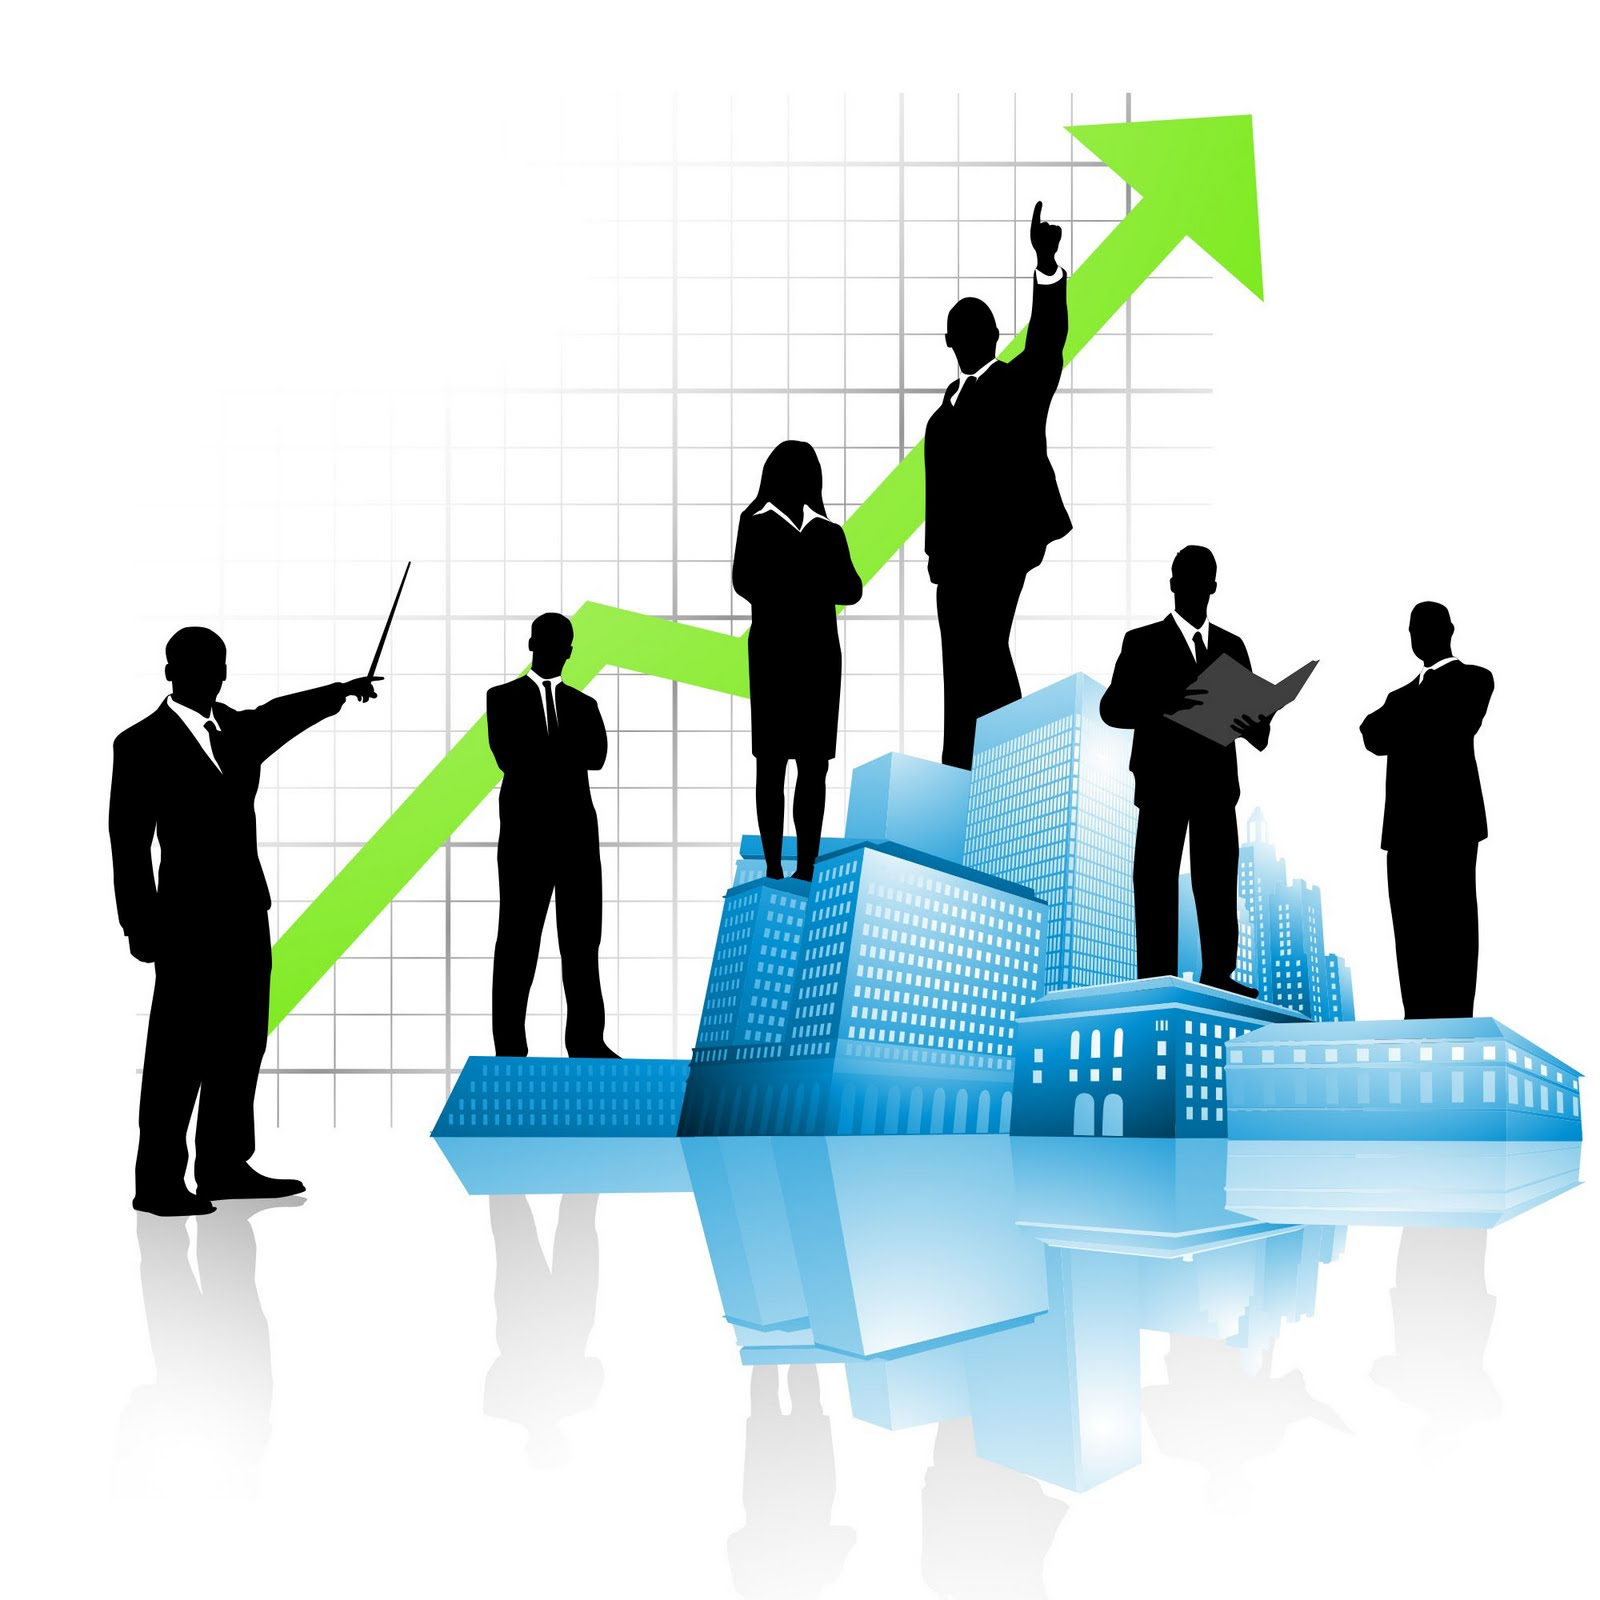
\includegraphics[height=\imageheight]{figure/corporate.jpg}


\includegraphics[height=\imageheight]{figure/education.jpg}
\end{center}
\end{column}

\mode<article>{\renewcommand{\imageheight}{0.2\textheight}}
\mode<presentation>{\renewcommand{\imageheight}{0.3\textheight}}

\begin{column}{0.23\textwidth}
\begin{center}
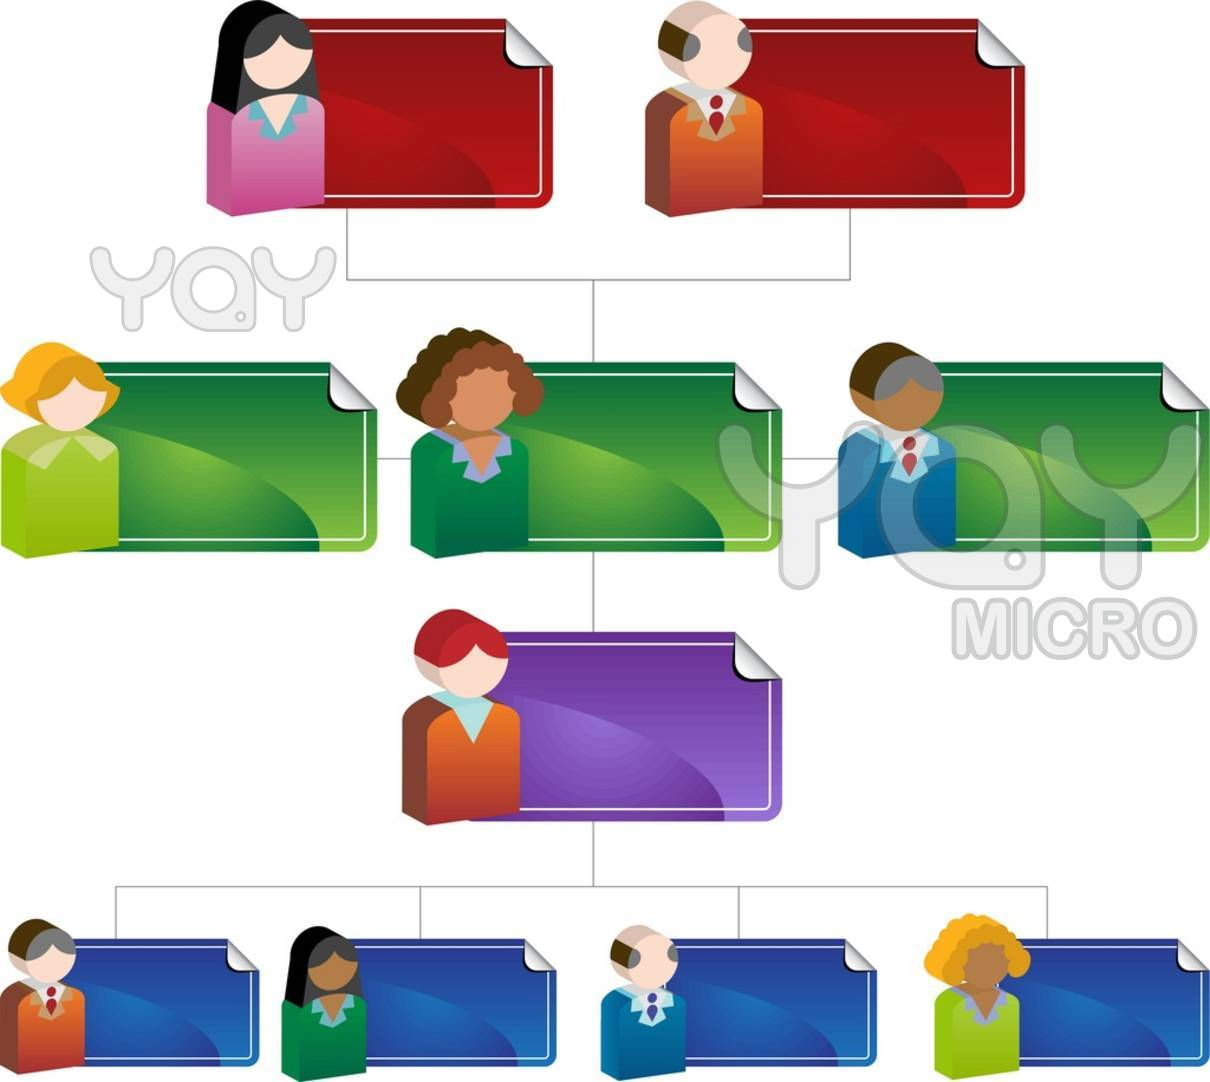
\includegraphics[height=\imageheight]{figure/orgchart.jpg}
\end{center}
\end{column}

\begin{column}{0.2\textwidth}
\begin{center}
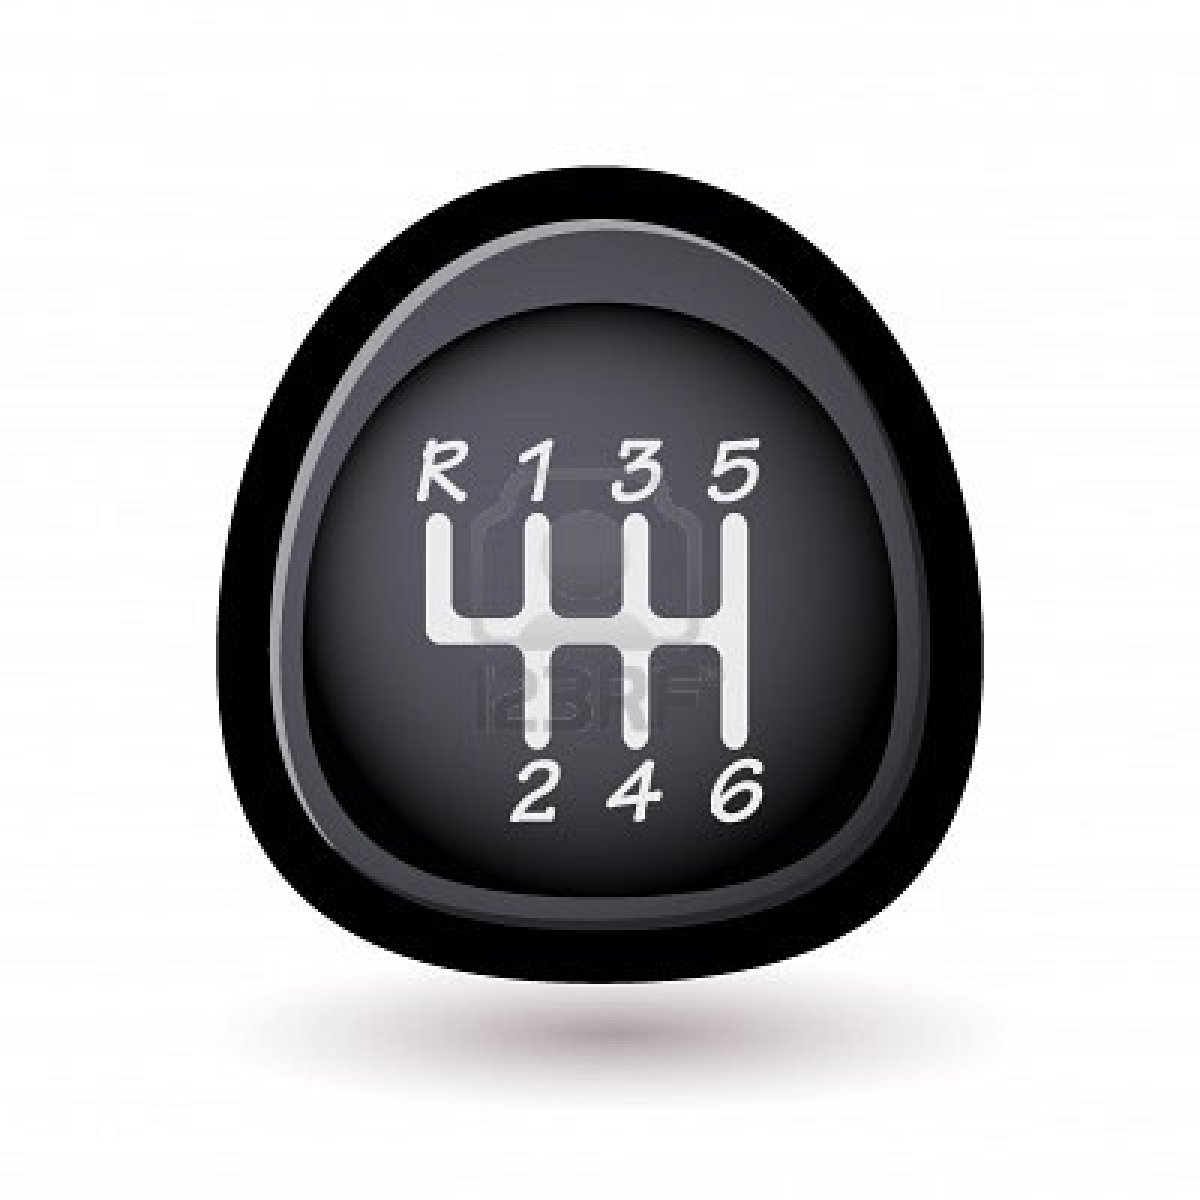
\includegraphics[height=\imageheight]{figure/shifter.jpg}
\end{center}
\end{column}

\begin{column}{0.23\textwidth}
\begin{center}

\includegraphics[height=\imageheight]{figure/operations.jpg}
\end{center}
\end{column}

\begin{column}{0.23\textwidth}
\begin{center}
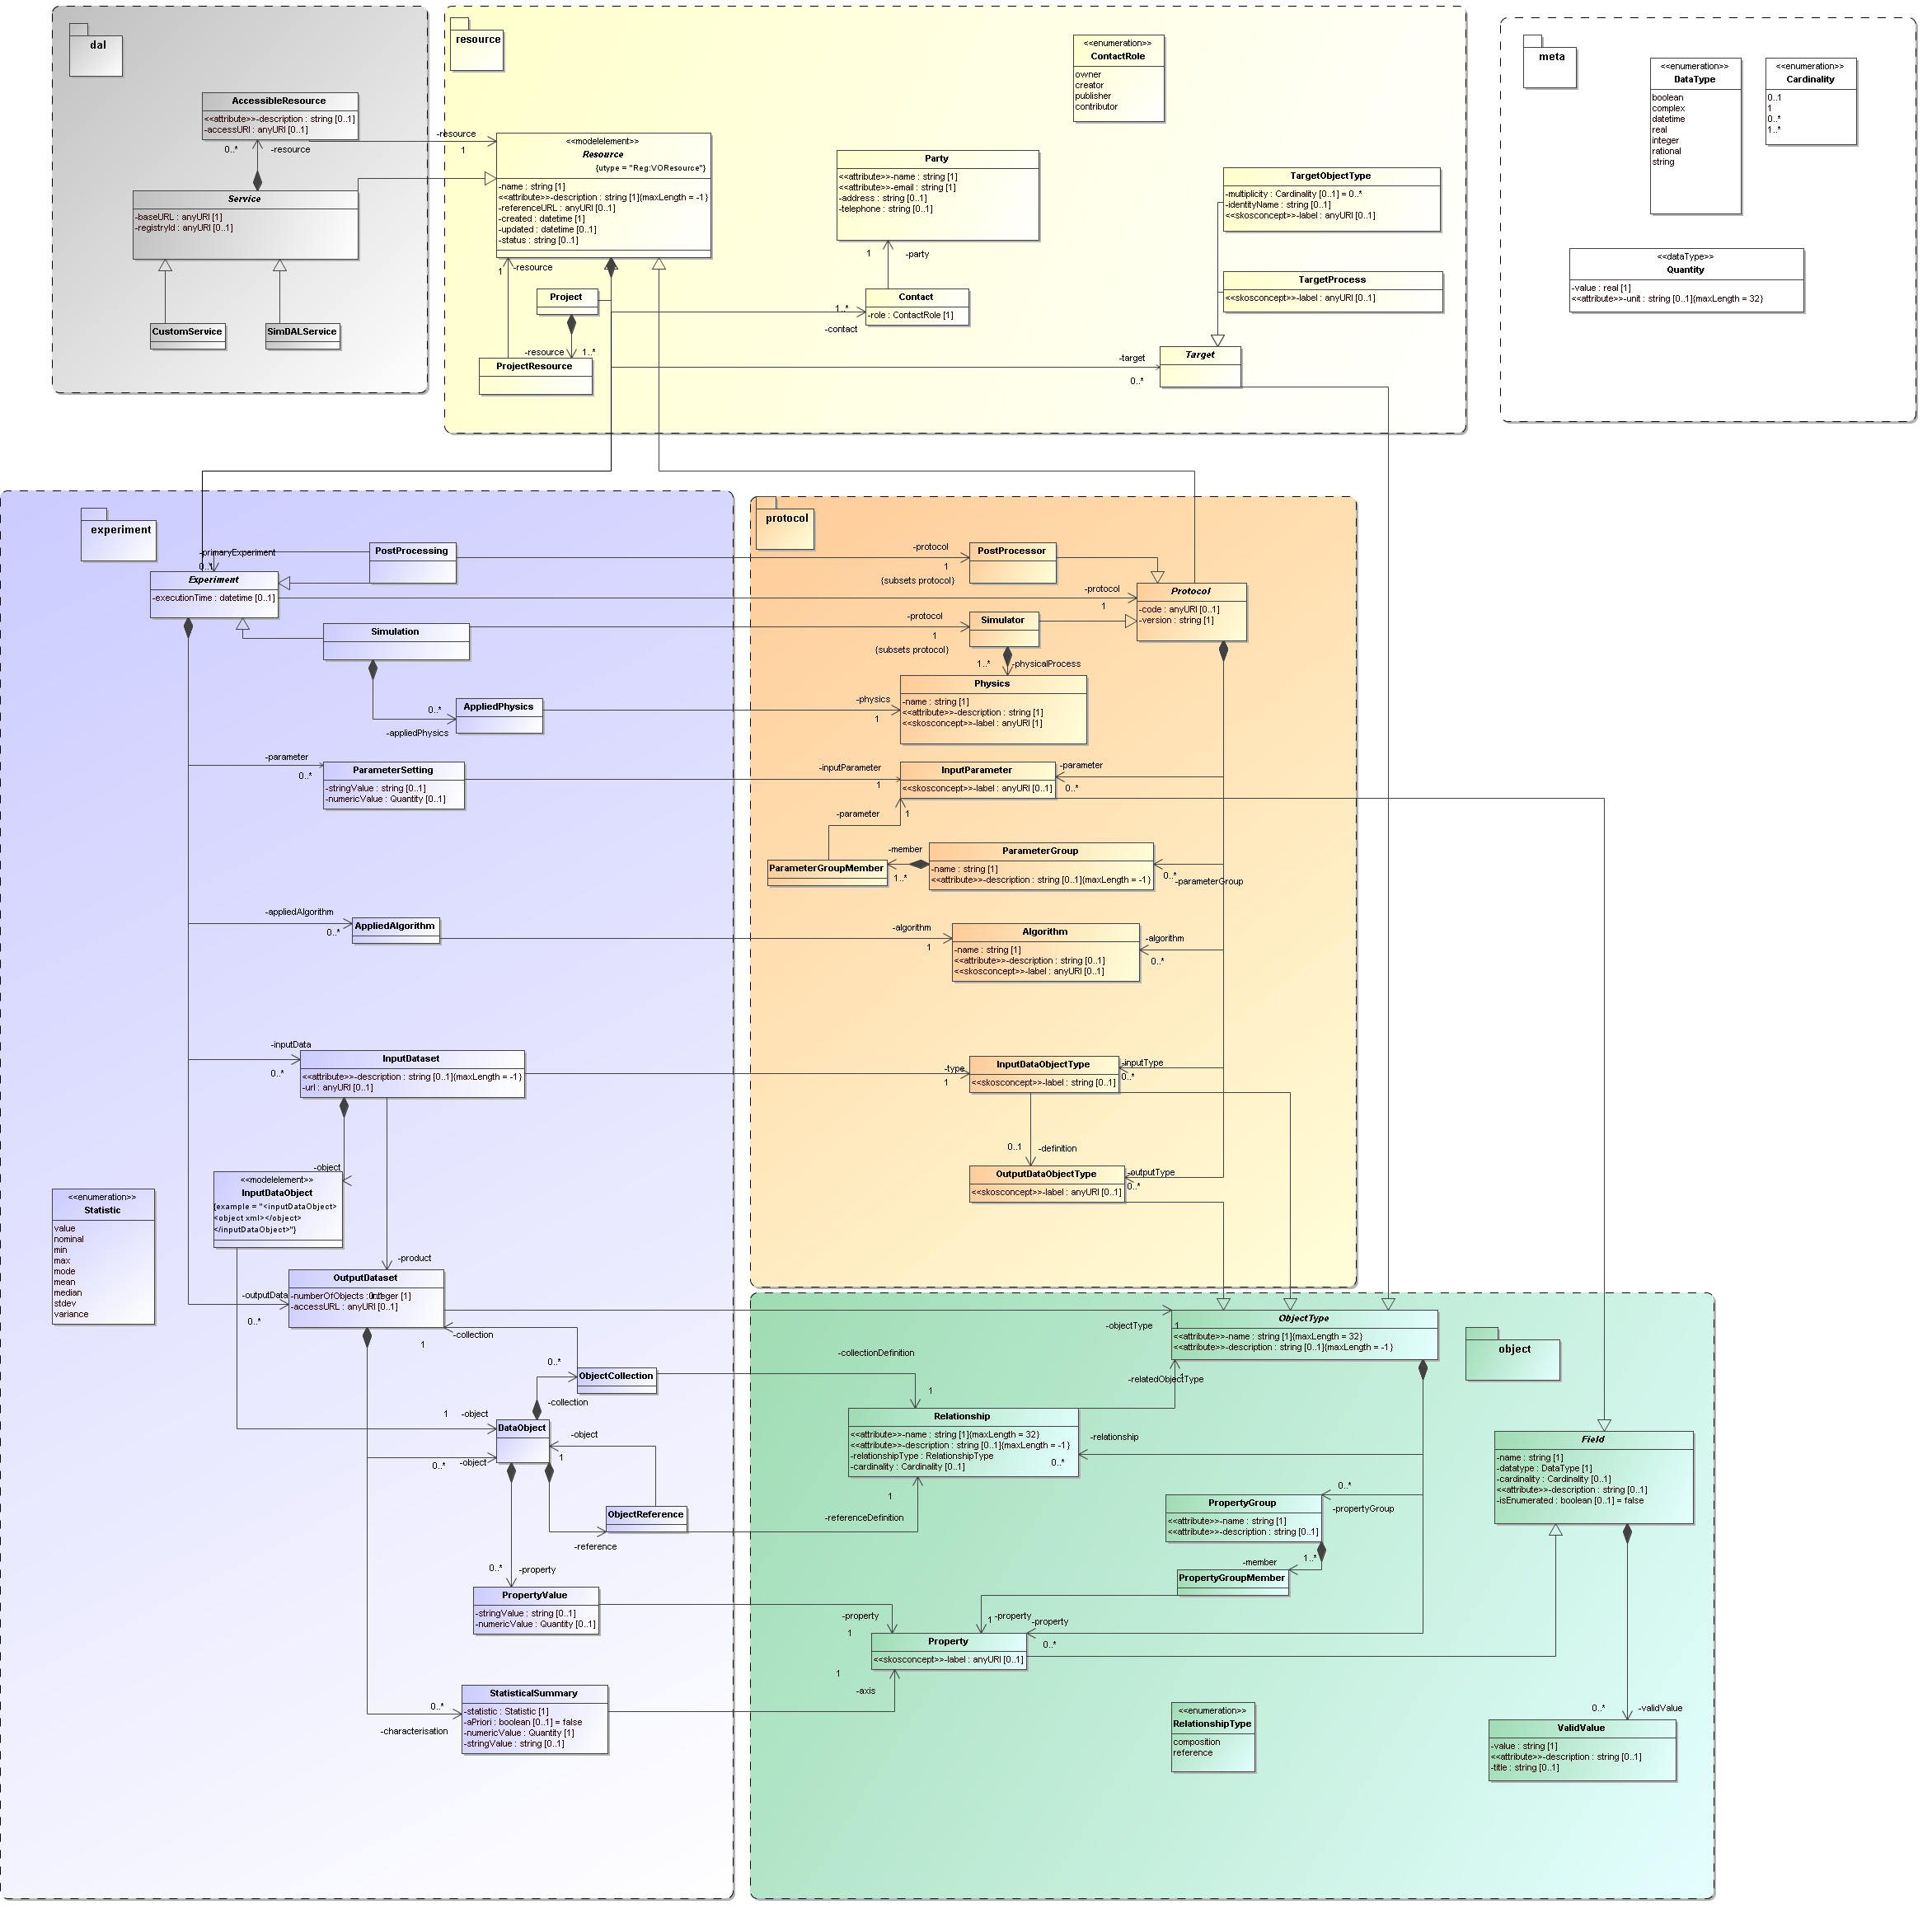
\includegraphics[height=\imageheight]{figure/function.png}
\end{center}
\end{column}

\end{columns}

\end{frame}
%%%%%%%%%%%%%%%%%%%%%%%%%%%%%%%%%%%%%%%%%%%%%%%%%%%%%%%%%%%%%%%%%%%%%%%%
\begin{frame}{Musa-1の手法でOPを得る手順(p118)}
\framesubtitle{Steps to develop OP, Musa-1}
\transboxout<1>
\transwipe<2->[direction=180]


\only<1>{ 1. 全種類の顧客に重みを付けて, 顧客のプロフィールを探し}
\only<2>{ 2. 一種の顧客の中関連するユーザーの型と彼らの相対使用率を定義し, 
    ユーザーのプロフィールを提示}
    \note<2>{顧客とユーザーの区別は, 顧客は製品を買う人, 
        ユーザーは製品を使う人}
\only<3>{ 3. よく使用される操作とそれの重みを見つけ,システムモード
    と関連プロフィールを定義}
\only<4>{ 4. システムモードを分析し, ハイレベルの機能とその関連するプロフィールを決定}
\only<5>{ 5. 細かい機能の使用率を決定}

\begin{columns}
\only<1,2>{
\begin{column}{0.5\textwidth}
\begin{center}
\mode<article>{\renewcommand{\imageheight}{0.07\textheight}}
\mode<presentation>{\renewcommand{\imageheight}{0.2\textheight}}

\includegraphics[height=\imageheight]{figure/goverment.png}

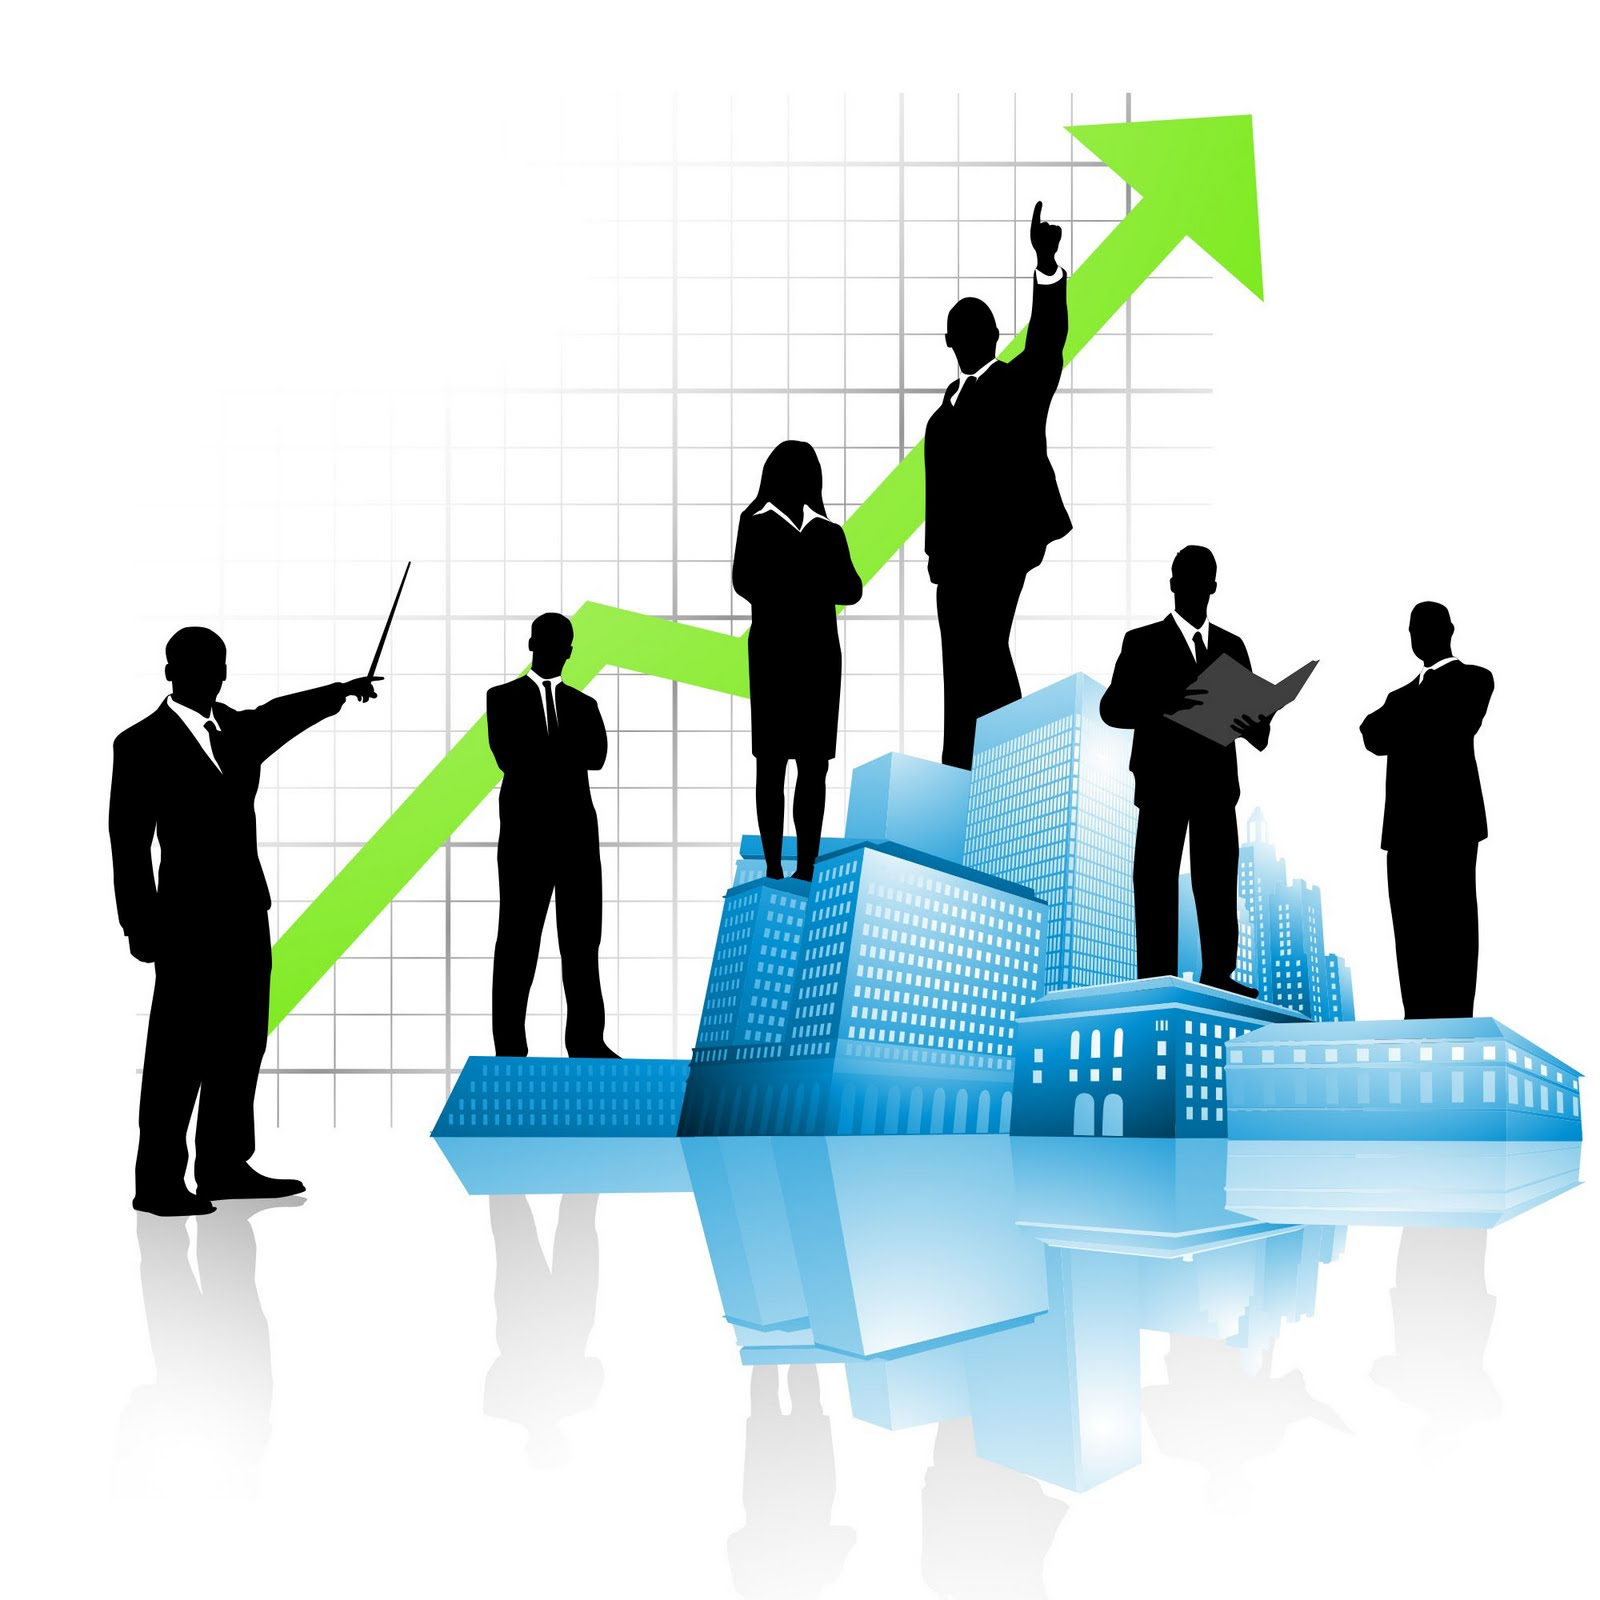
\includegraphics[height=\imageheight]{figure/corporate.jpg}


\includegraphics[height=\imageheight]{figure/education.jpg}
\end{center}
\end{column}
}

\mode<article>{\renewcommand{\imageheight}{0.2\textheight}}
\mode<presentation>{\renewcommand{\imageheight}{0.6\textheight}}

\only<2,3>{
\begin{column}{0.5\textwidth}
\begin{center}
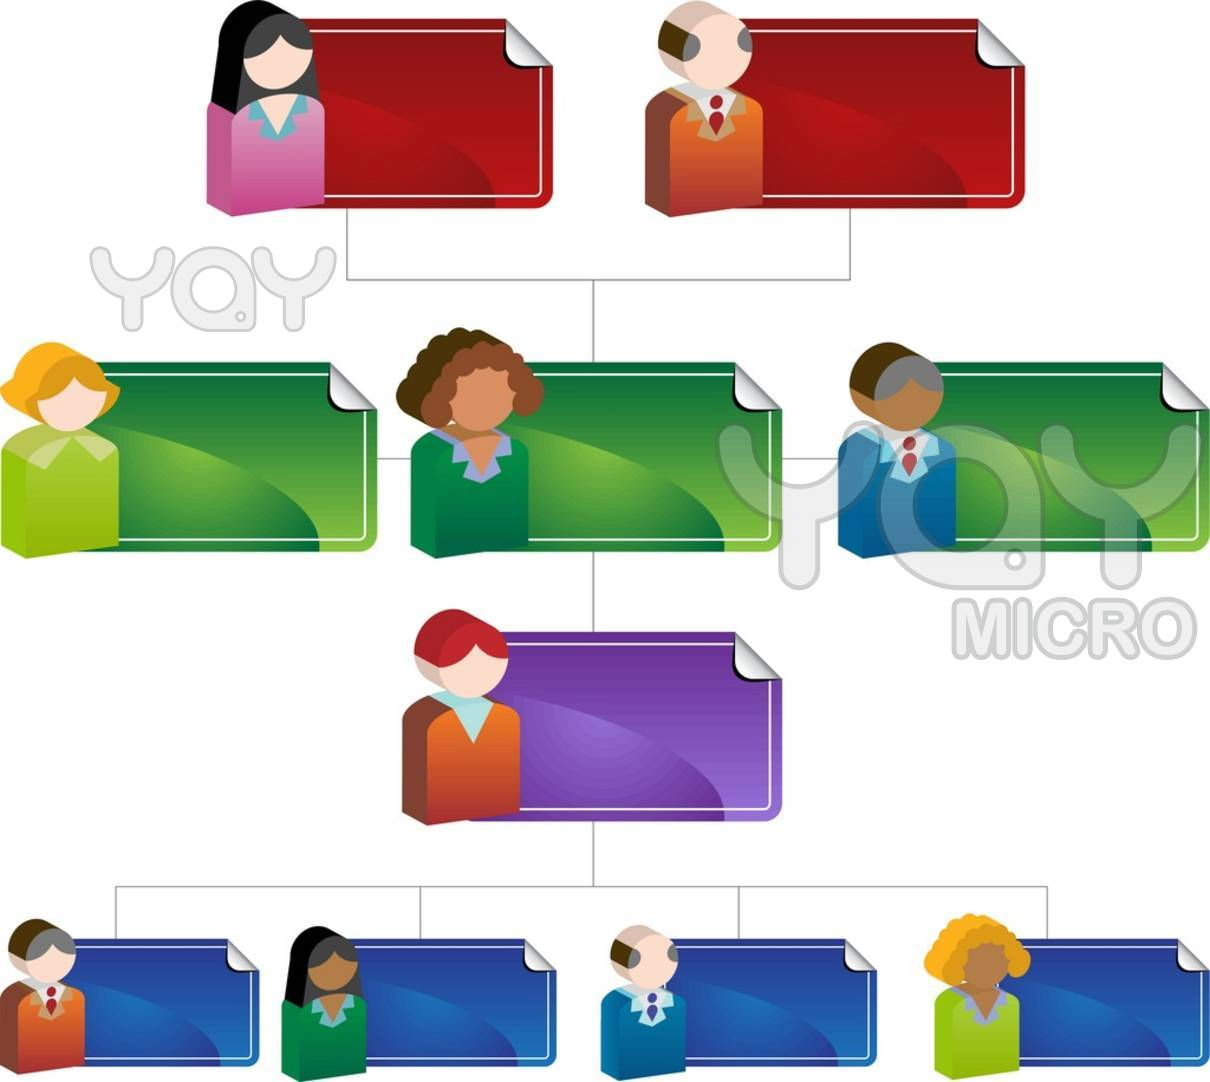
\includegraphics[height=\imageheight]{figure/orgchart.jpg}
\end{center}
\end{column}
}

\only<3,4>{
\begin{column}{0.5\textwidth}
\begin{center}
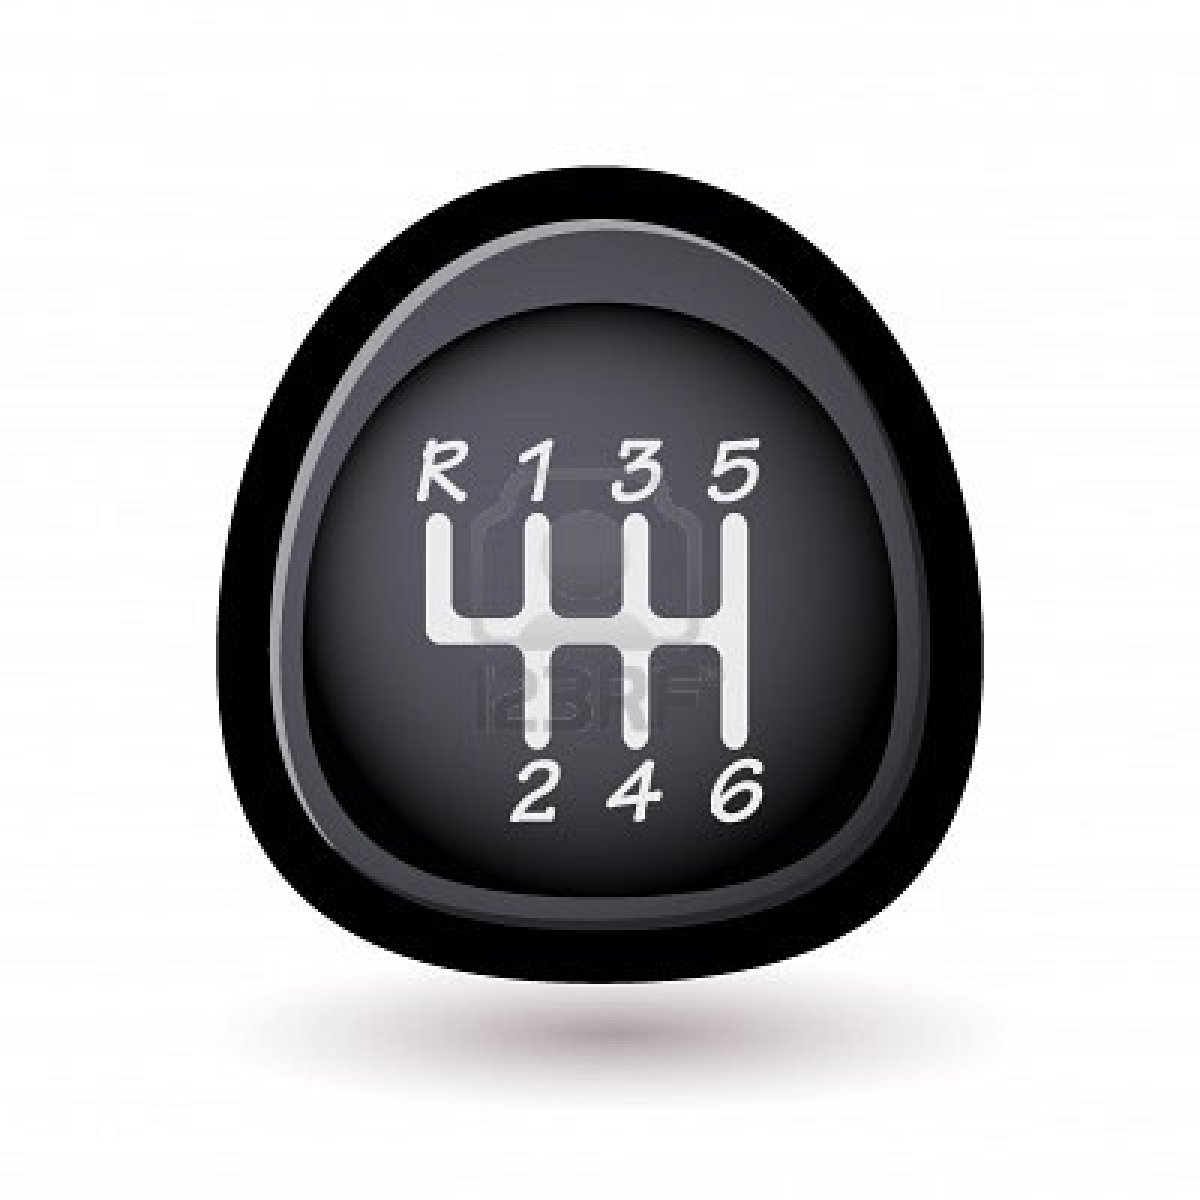
\includegraphics[height=\imageheight]{figure/shifter.jpg}
\end{center}
\end{column}
}

\only<4,5>{
\begin{column}{0.5\textwidth}
\begin{center}

\includegraphics[height=\imageheight]{figure/operations.jpg}
\end{center}
\end{column}
}

\only<5>{
\begin{column}{0.5\textwidth}
\begin{center}
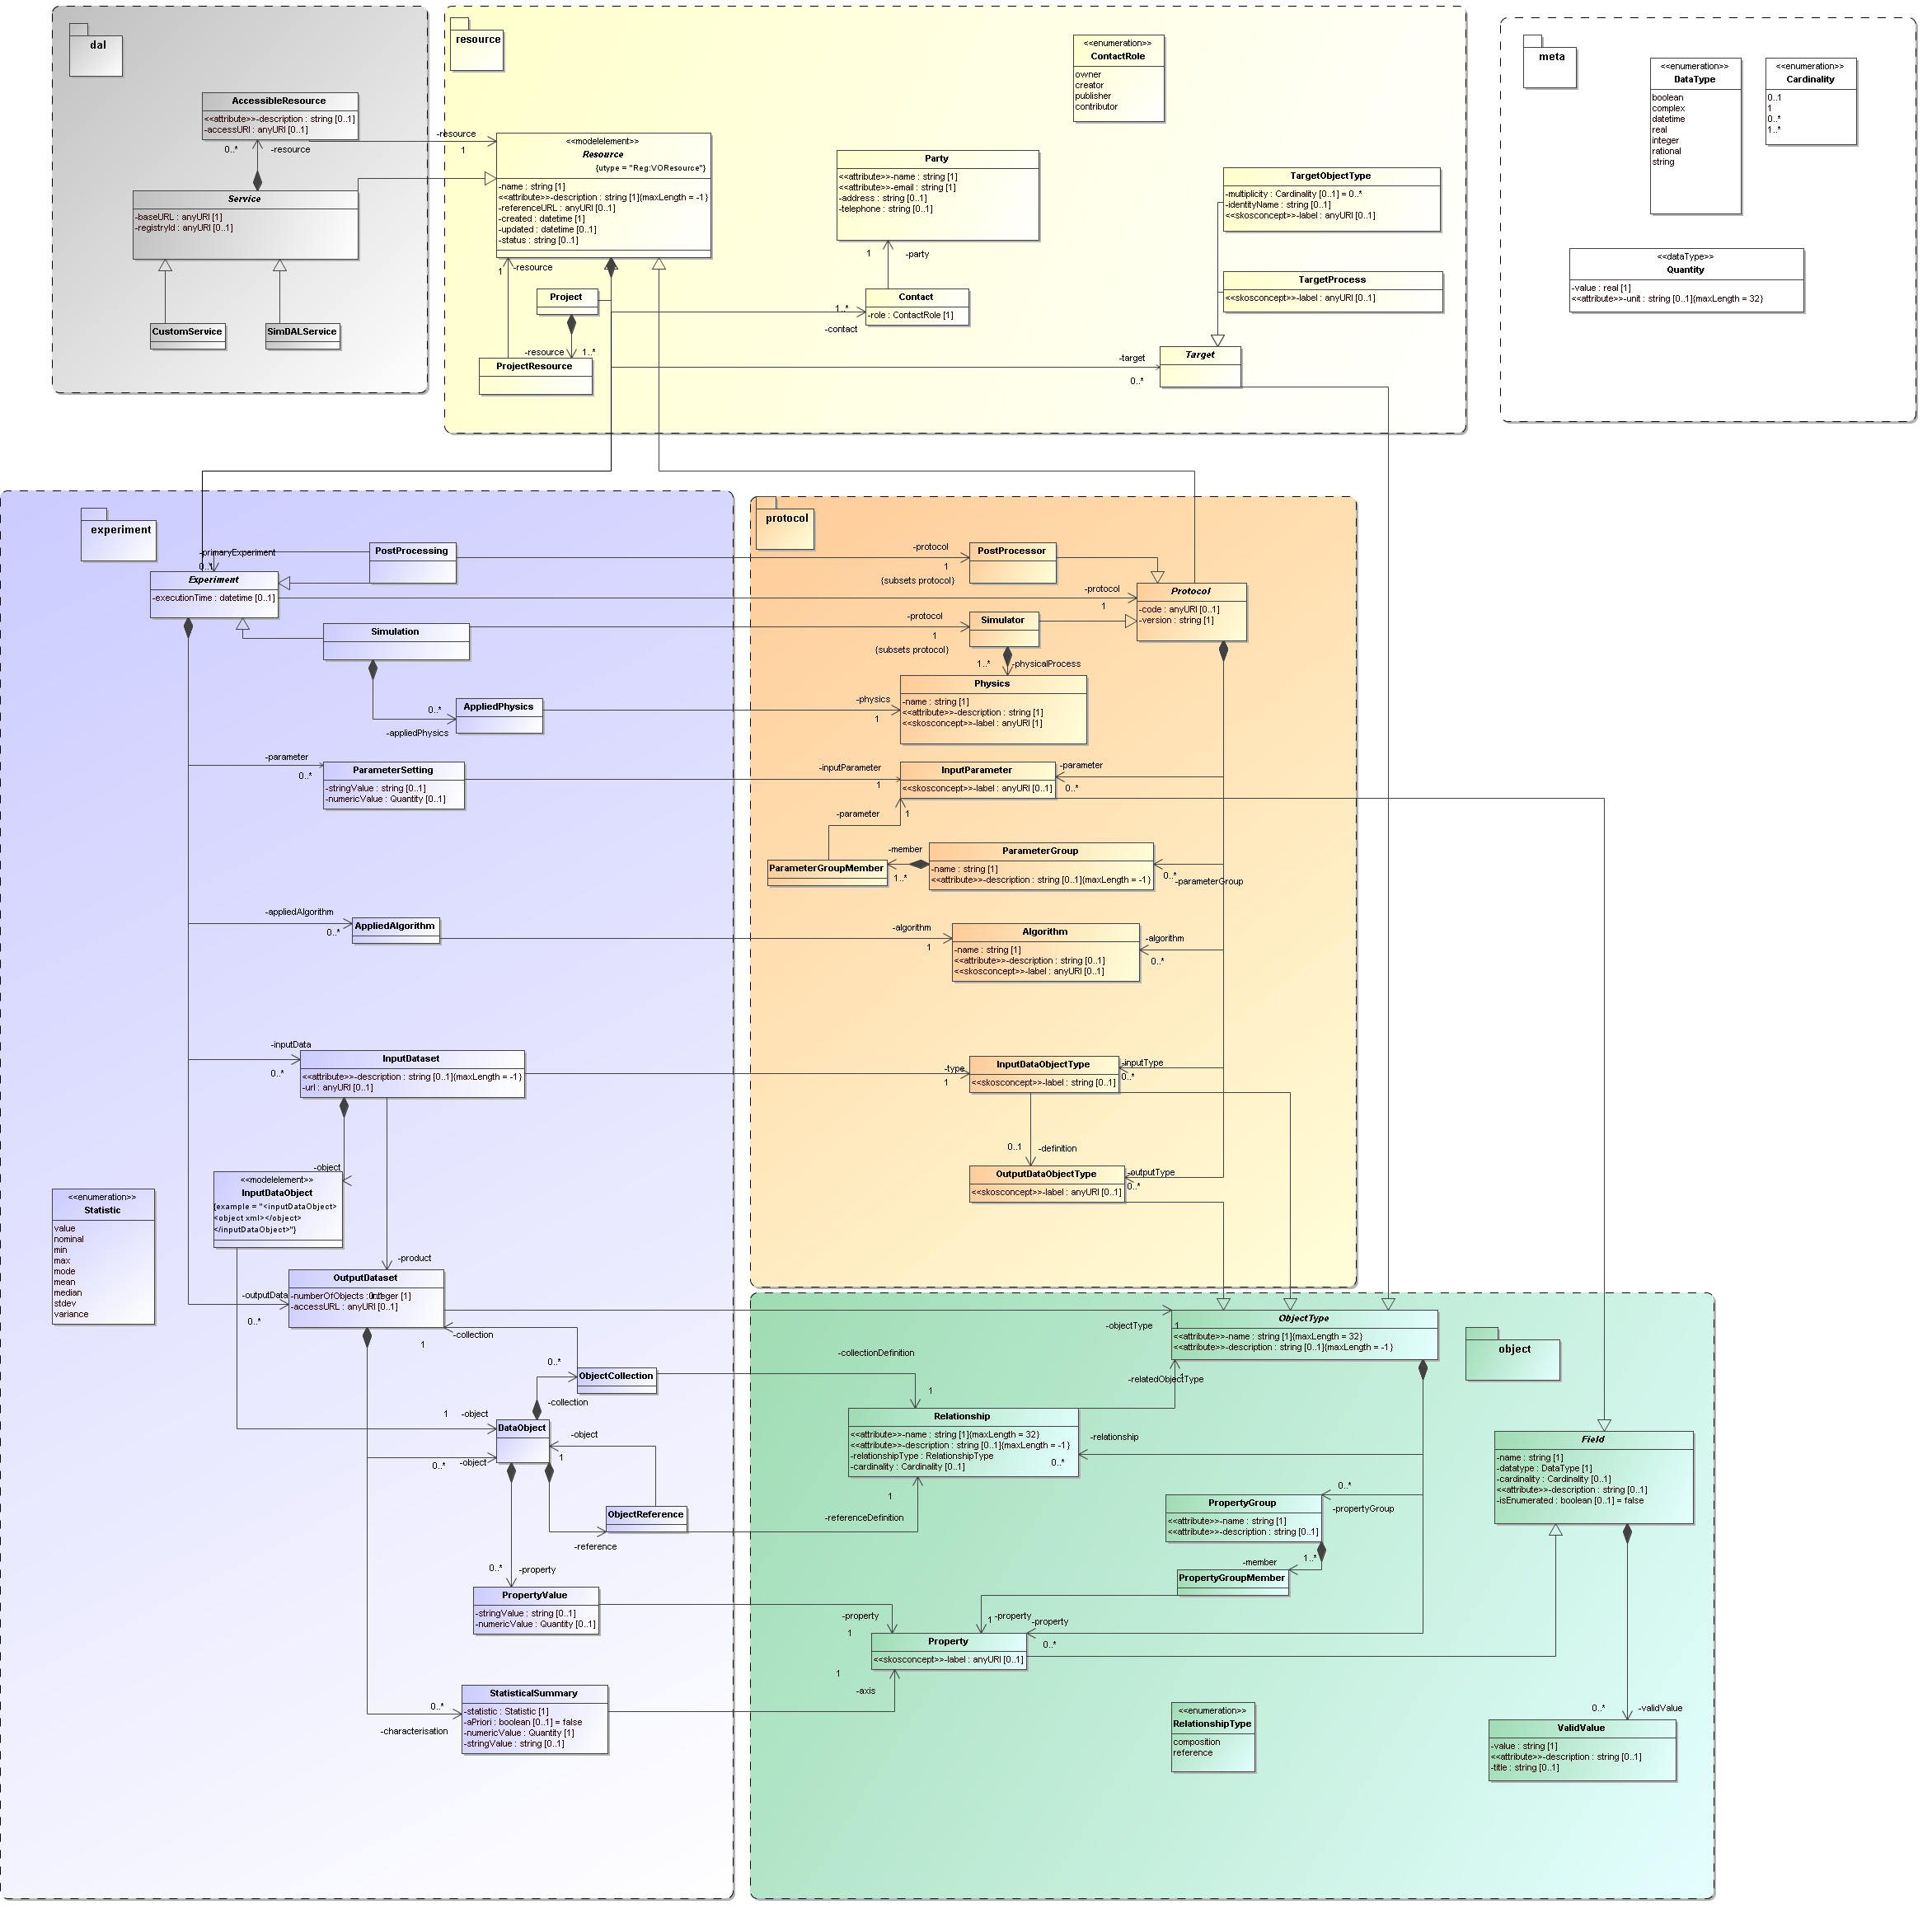
\includegraphics[height=\imageheight]{figure/function.png}
\end{center}
\end{column}
}

\end{columns}
\end{frame}


%%%%%%%%%%%%%%%%%%%%%%%%%%%%%%%%%%%%%%%%%%%%%%%%%%%%%%%%%%%%%%%%%%%%%%%%
\begin{frame}{Musa-1:例(p118)}
\framesubtitle{Sample for Musa-1}
\begin{figure}
\subfloat[顧客操作プロフィールの例]{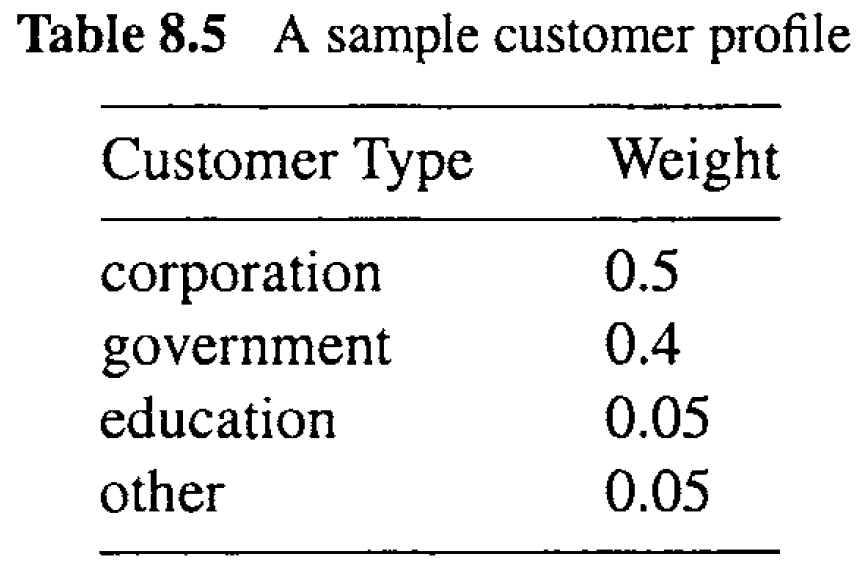
\includegraphics[height=\imageheight]{figure/samplecustomerprofile.png}}
\subfloat[ユーザー操作プロフィールの例]{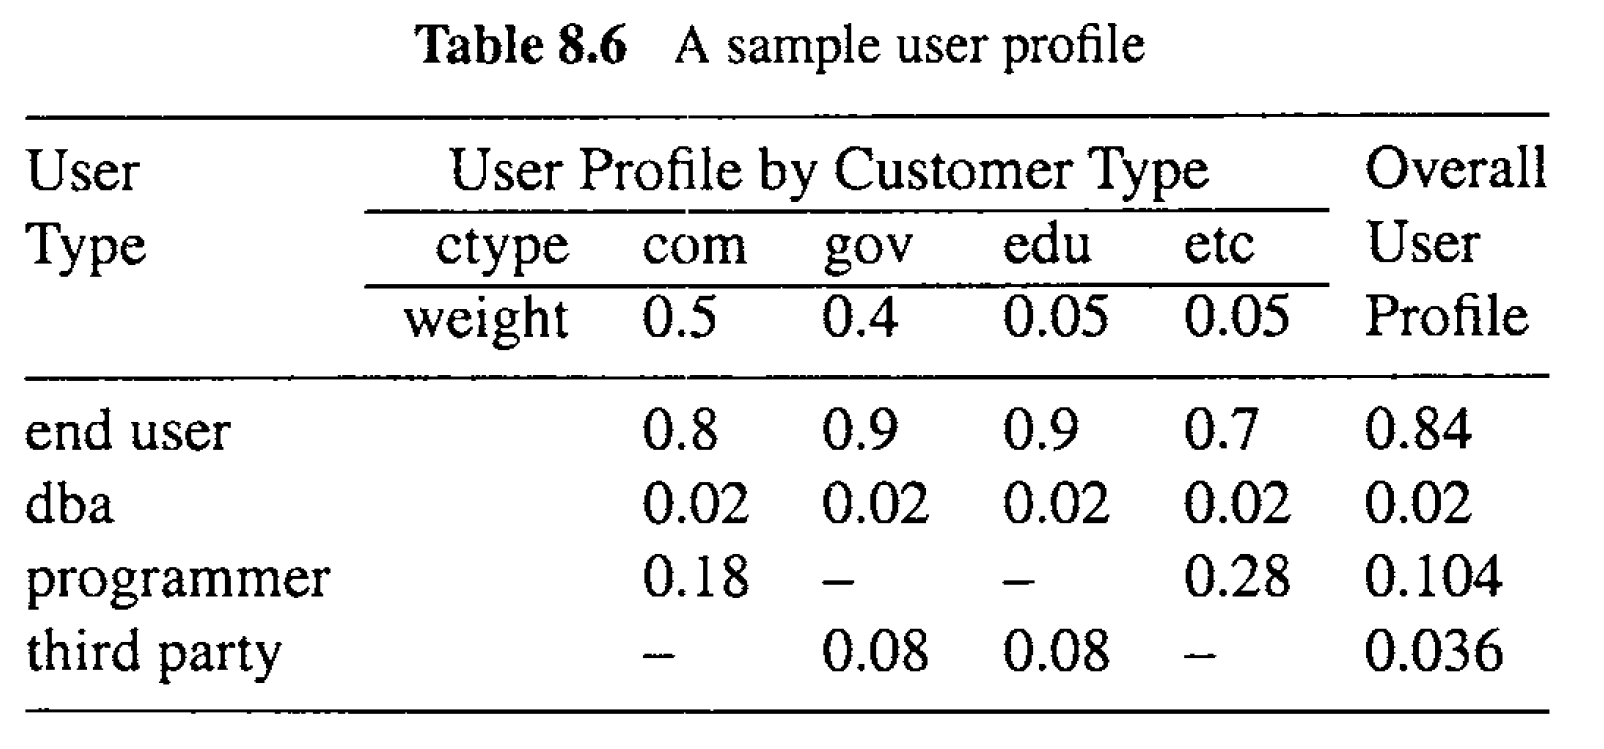
\includegraphics[height=\imageheight]{figure/sampleuserprofile.png}}
\caption{操作プロフィールをMusa-1で開発する例}
\end{figure}
\end{frame}
%%%%%%%%%%%%%%%%%%%%%%%%%%%%%%%%%%%%%%%%%%%%%%%%%%%%%%%%%%%%%%%%%%%%%%%%
\begin{frame}{一貫性があるOPの計算(p119)}
\framesubtitle{Calculate Profile for Uniform Operational Stages}
もし一つの操作が二つの段階(A, B)に分かれて, それぞれのプロフィール
\[p_i=prob(A=A_i)\]
\[p_j=prob(B=B_j)\]

操作全体のプロフィール

\[p_{ij}=prob(A=A_i,B=B_j)=p_i \times p_j\]
\end{frame}
%%%%%%%%%%%%%%%%%%%%%%%%%%%%%%%%%%%%%%%%%%%%%%%%%%%%%%%%%%%%%%%%%%%%%%%%
\subsection{8.4.3 Musa-2操作プロフィールの開発過程}
\begin{frame}{Musa-2 OPの開発過程(p120)}
\framesubtitle{OP development procedure: Musa-2}
\begin{definationfc}[Musa-2]
一つユーザーに対して単一な操作プロフィール

もっと小さいデータソースに適用
\end{definationfc}

\pause
\begin{enumerate}
\item 操作のイニシエータ(initiator)を決定
\item 表現の形式を決定:\alert<3->{表か図か}
\item 操作配列を決定
\item 発生率の測定単位を決定
\item 発生する可能性を決め
\end{enumerate}
\end{frame}
%%%%%%%%%%%%%%%%%%%%%%%%%%%%%%%%%%%%%%%%%%%%%%%%%%%%%%%%%%%%%%%%%%%%%%%%
\begin{frame}{Musa-2 表現の形式:表(p120)}
\framesubtitle{Musa-2 Representation: Tabular}
\begin{center}
\includegraphics[width=0.8\textwidth,page=51]{figure/include.pdf}
\end{center}
\end{frame}
%%%%%%%%%%%%%%%%%%%%%%%%%%%%%%%%%%%%%%%%%%%%%%%%%%%%%%%%%%%%%%%%%%%%%%%%
\begin{frame}{Musa-2 表現の形式:図(p121)}
\framesubtitle{Musa-2 Representation: Graphical}
\begin{center}
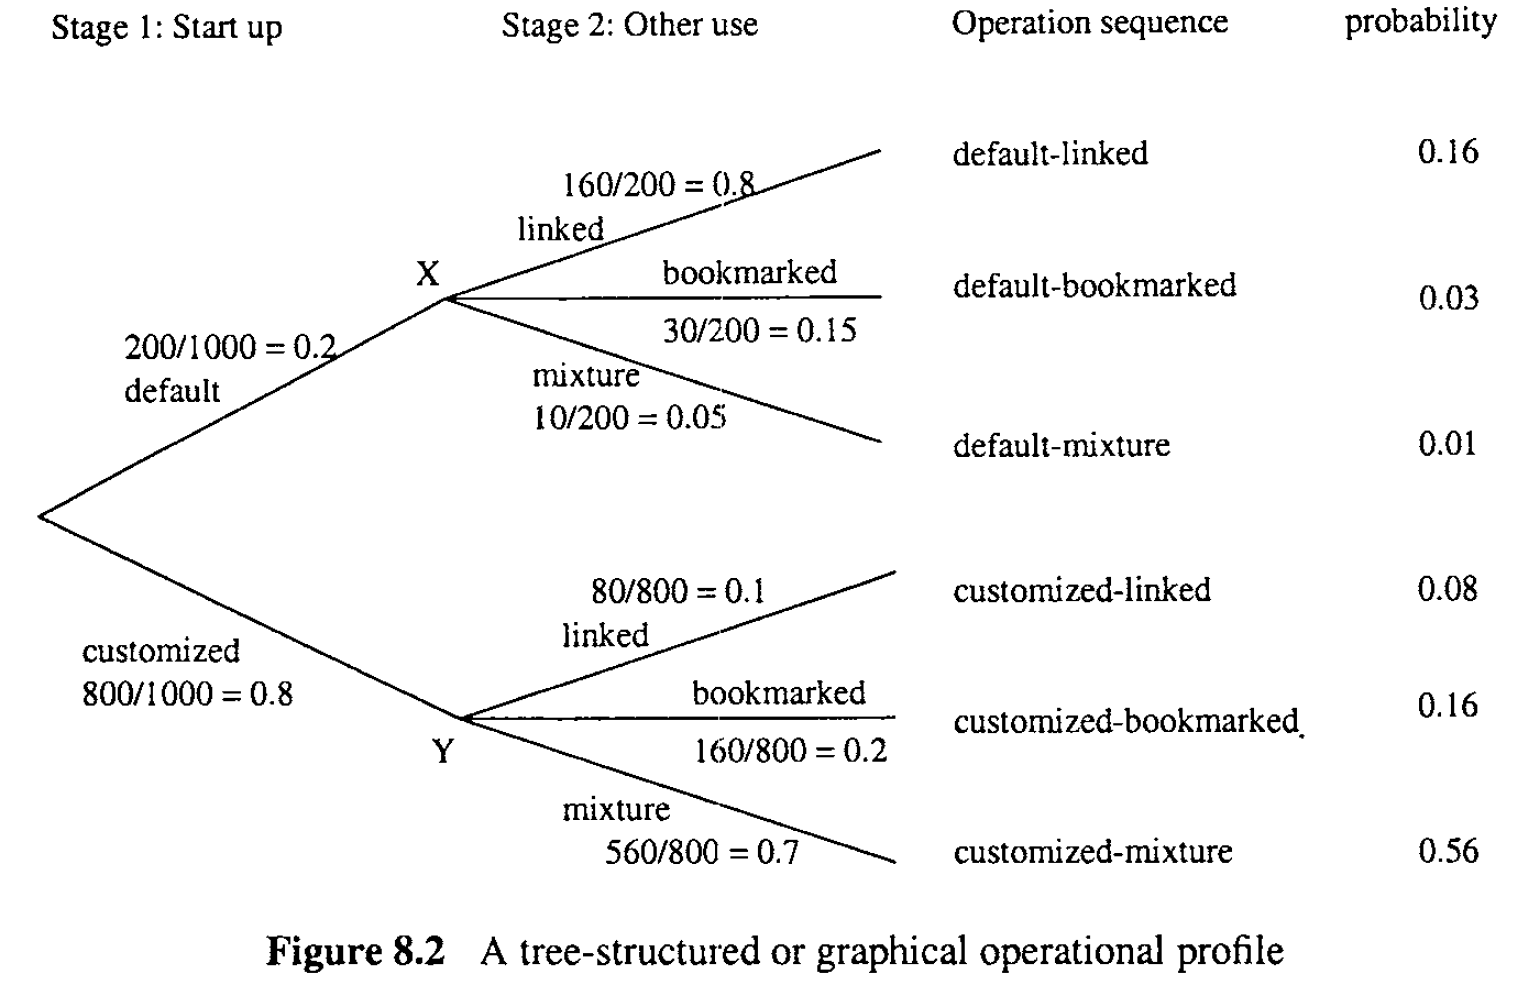
\includegraphics[width=\textwidth,height=0.8\textheight,keepaspectratio]{figure/graphical.png}
\end{center}
\end{frame}
%%%%%%%%%%%%%%%%%%%%%%%%%%%%%%%%%%%%%%%%%%%%%%%%%%%%%%%%%%%%%%%%%%%%%%%%
\section{8.5 Case Study: 交換支援ソフトウェアに使うOP}
\subsection{8.5.1 背景と参加者}
\begin{frame}{交換支援システムの背景(p121)}
\framesubtitle{Background for Cartridge Support System}
Lockheed Martin戦術航空機(Tactical Aircraft)\note{航空機:こうくうき}
会社(LMTAS)が開発した, 航空機要員に使われて, 任務の計画の媒介を交換するの
支援システム(Cartridge Support Software, CSS)

\begin{columns}
\begin{column}{0.6\textwidth}
\begin{center}
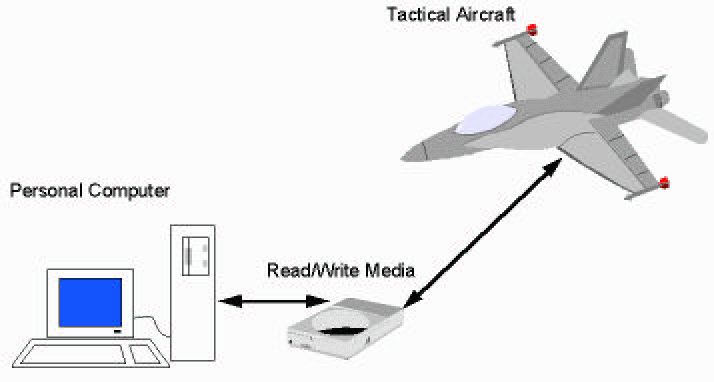
\includegraphics[width=\textwidth,height=0.5\textheight,keepaspectratio]{figure/CSS.png}
\end{center}
\end{column}
\begin{column}{0.4\textwidth}
\begin{center}
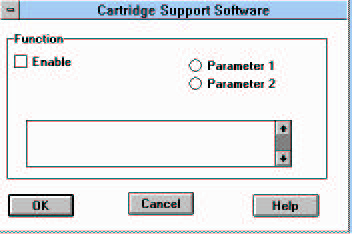
\includegraphics[width=\textwidth,height=0.5\textheight,keepaspectratio]{figure/CSSdialog.png}
\end{center}
\end{column}
\end{columns}

\note[item]{航空機要員は媒介を使って、航空機に乗せているコンピューターに
データをアップロードする。航空機要員で任務の計画をロートできるという能力は
パイロットにとって非常に大事、それがないと、パイロットは複雑なコントロール・パネル
で必死に様々なデータを設定しなければならない。CSSを使ったら、パソコンをGUIから、
航空機要員は任務の計画を立つ操作は簡単に、効率的になる。}

\end{frame}
%%%%%%%%%%%%%%%%%%%%%%%%%%%%%%%%%%%%%%%%%%%%%%%%%%%%%%%%%%%%%%%%%%%%%%%%
\begin{frame}{CSSのOPを開発する参加者(p122)}
\framesubtitle{Participants in Developing OP of CSS}
\note{
操作プロフィール開発を導入した
\begin{itemize}
\item ユーザーの視点からCSSをもっと理解するために
\item 高級機能を着目してテストするために
\end{itemize}
}

参加者\cite{chruscielski1997operational}は
\begin{itemize}
\item Software Product Manager
    \note[item]{SPM:責任はCSS製品の機能の計画して、売り出す。
            SPMはユーザーの入力から、操作プロフィールへの
            交流を指導者です。}
\item Software Test Engineers
    \note[item]{STE:責任は各操作ごとにテスト可能な入力状態を把握する。}
\item System Engineers
    \note[item]{SE:責任はシステムの要求やハイレベルの設計、
        交付(こうふ)可能な機能等を提出し、テストに確認します}
\end{itemize}

\begin{thebibliography}{Chruscielski and Tian(1997)}
\bibitem[Chruscielski and Tian(1997)]{chruscielski1997operational}
K.~Chruscielski and J.~Tian, ``An operational profile for the cartridge support
  software,'' in \emph{PROCEEDINGS The Eighth International Symposium On
  Software Reliability Engineering}.\hskip 1em plus 0.5em minus 0.4em\relax
  IEEE, 1997, pp. 203--212.
\end{thebibliography}

\note[item]{レポートを書いた二人はSMU(南メソジスト大学)に
    「ソフトウェアテストと品質保証」を教える先生。}
\end{frame}

%%%%%%%%%%%%%%%%%%%%%%%%%%%%%%%%%%%%%%%%%%%%%%%%%%%%%%%%%%%%%%%%%%%%%%%%
\subsection{8.5.2 五つのステップでOP開発}
\begin{frame}{Step 1\&2: 顧客とユーザー(p122)}
\framesubtitle{Step 1\&2: Customers \& Users}
CSSの顧客は空軍\note[item]{空軍:くうぐん}
\note[item]{内部顧客:航空機システムテスト者、飛行テスト者もいるが、
    基本の操作は一緒ですから、区別しない、重みをつけない}
\begin{overlayarea}{\textwidth}{0.7\textheight}
\only<1>{
    \begin{center}
    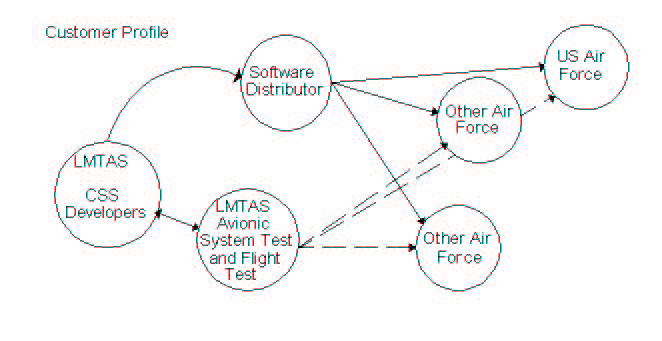
\includegraphics[width=\textwidth,height=0.8\textheight,keepaspectratio]{figure/CSScustomer.png}
    \end{center}
}
\only<2->{
\transfade[duration=0.1]
ユーザーの型は
\begin{overlayarea}{\textwidth}{0.6\textheight}
\only<2>{
\begin{enumerate}
\item 空軍のパイロット
    \note[item]{パイロット:直接に関係する人、あんまり操作しない}
\item 飛行テスト支援者
    \note[item]{Flight Test Support: 任務計画中にCSSを使う人}
\item 航空機システムテスト者
    \note[item]{航空機の中の全部載せているパソコンを管理、設置する人}
\item システム管理者
    \note[item]{この機能はパイロットに実行しているから、パイロットに合併する}
\end{enumerate}
}
\only<3>{
    \begin{figure}
    \begin{center}
    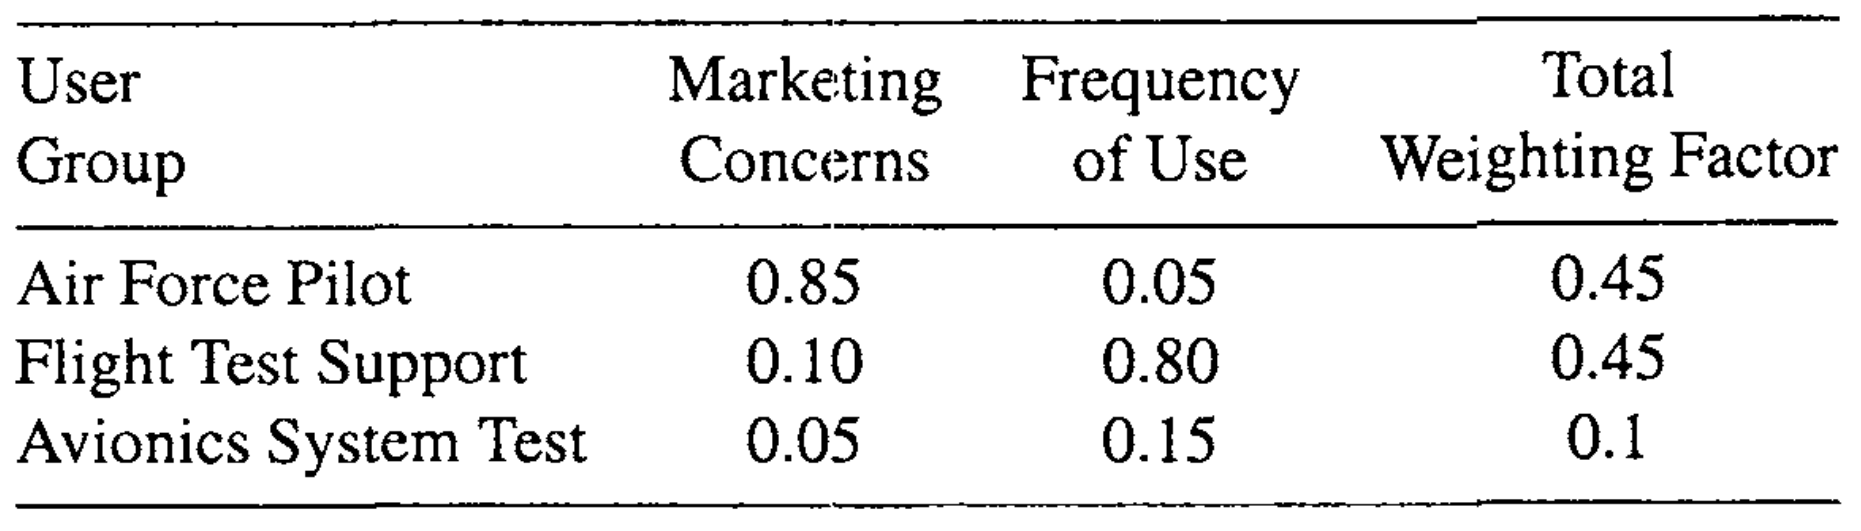
\includegraphics[width=\textwidth,height=\imageheight,keepaspectratio]{figure/CSSuser.png}
    \caption{CSSユーザー・プロフィール}
    \end{center}
    \end{figure}
}
\end{overlayarea}
}
\end{overlayarea}
\end{frame}

%%%%%%%%%%%%%%%%%%%%%%%%%%%%%%%%%%%%%%%%%%%%%%%%%%%%%%%%%%%%%%%%%%%%%%%%
\begin{frame}{Step 3: システム・モード(p123)}
\framesubtitle{Step 3: System Modes}
CSSに見つけたシステム・モードは三種類に分かれています:
\begin{enumerate}
\item 飛行前の任務計画
\item 航空機システムテスト
\item システム管理
\end{enumerate}
操作分析によると, この三つは区別しない。
\end{frame}
%%%%%%%%%%%%%%%%%%%%%%%%%%%%%%%%%%%%%%%%%%%%%%%%%%%%%%%%%%%%%%%%%%%%%%%%
\begin{frame}{Step 4\&5: 機能と操作(p123)}
\framesubtitle{Step 4\&5: High-level functions and low-level operations}
\begin{center}
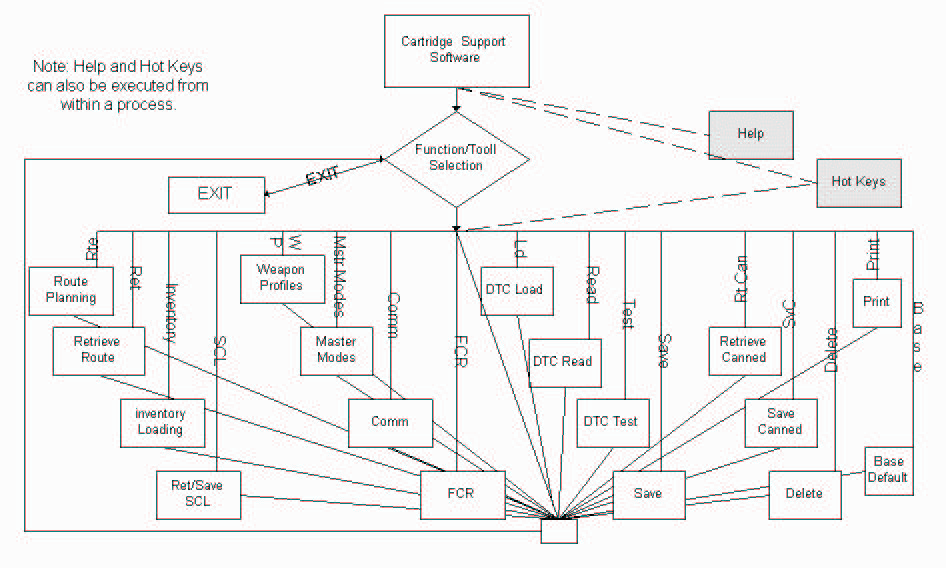
\includegraphics[width=\textwidth,height=0.7\textheight,keepaspectratio]{figure/CSSflow.png}
\end{center}
\end{frame}
%%%%%%%%%%%%%%%%%%%%%%%%%%%%%%%%%%%%%%%%%%%%%%%%%%%%%%%%%%%%%%%%%%%%%%%%
\begin{frame}{パイロットのOP}
\framesubtitle{OP: Pilot}
\begin{center}
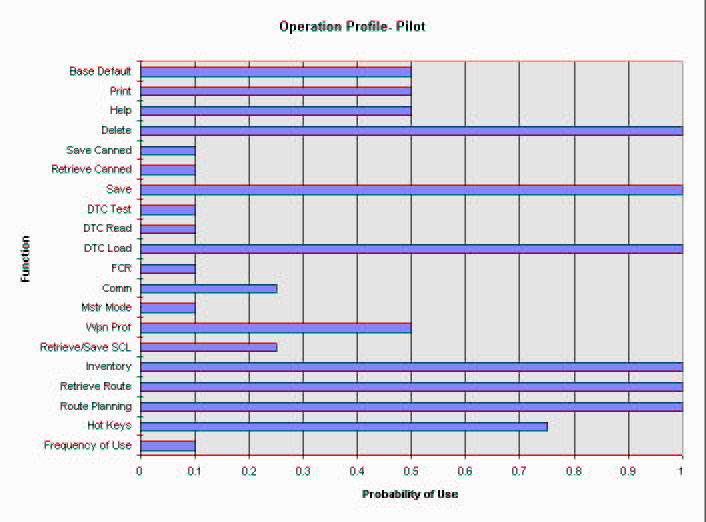
\includegraphics[width=\textwidth,height=0.7\textheight,keepaspectratio]{figure/OPpilot.png}
\end{center}
\end{frame}
%%%%%%%%%%%%%%%%%%%%%%%%%%%%%%%%%%%%%%%%%%%%%%%%%%%%%%%%%%%%%%%%%%%%%%%%
\begin{frame}{飛行テスト支援者のOP}
\framesubtitle{OP: Flight Test Support}
\begin{center}
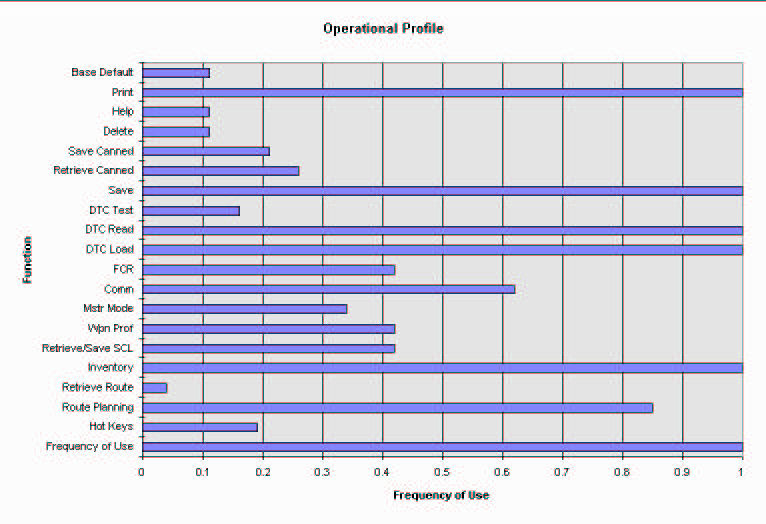
\includegraphics[width=\textwidth,height=0.7\textheight,keepaspectratio]{figure/OPfts.png}
\end{center}
\end{frame}
%%%%%%%%%%%%%%%%%%%%%%%%%%%%%%%%%%%%%%%%%%%%%%%%%%%%%%%%%%%%%%%%%%%%%%%%
\begin{frame}{システム・テスト者のOP}
\framesubtitle{OP: System Test}
\begin{center}
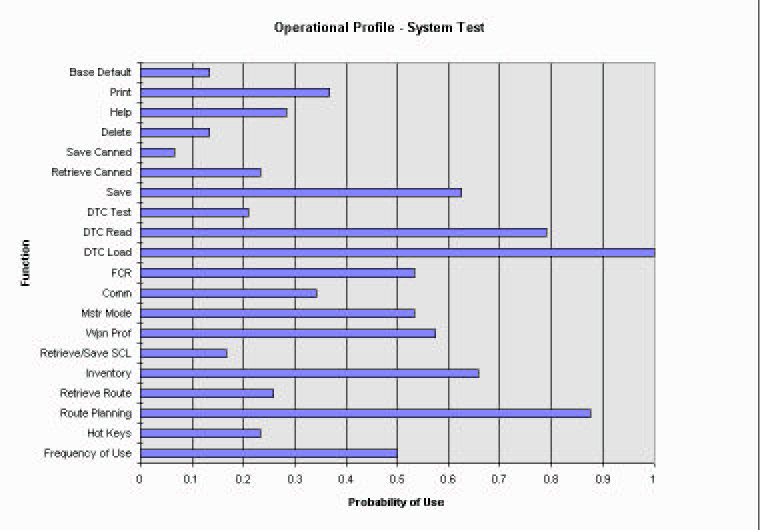
\includegraphics[width=\textwidth,height=0.7\textheight,keepaspectratio]{figure/OPst.png}
\end{center}
\end{frame}
%%%%%%%%%%%%%%%%%%%%%%%%%%%%%%%%%%%%%%%%%%%%%%%%%%%%%%%%%%%%%%%%%%%%%%%%
\begin{frame}{全部のOP}
\framesubtitle{OP: Comprehensive}
\begin{center}
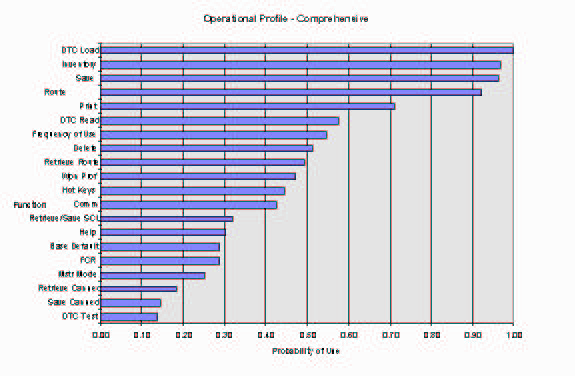
\includegraphics[width=\textwidth,height=0.7\textheight,keepaspectratio]{figure/OPcompre.png}
\end{center}
\end{frame}
%%%%%%%%%%%%%%%%%%%%%%%%%%%%%%%%%%%%%%%%%%%%%%%%%%%%%%%%%%%%%%%%%%%%%%%%
%%%%%%%%%%%%%%%%%%%%%%%%%%%%%%%%%%%%%%%%%%%%%%%%%%%%%%%%%%%%%%%%%%%%%%%%

\begin{frame}{CSS使用率よる機能の分類(p124)}
\framesubtitle{CSS functions classified according to usage probabilities}
\begin{center}
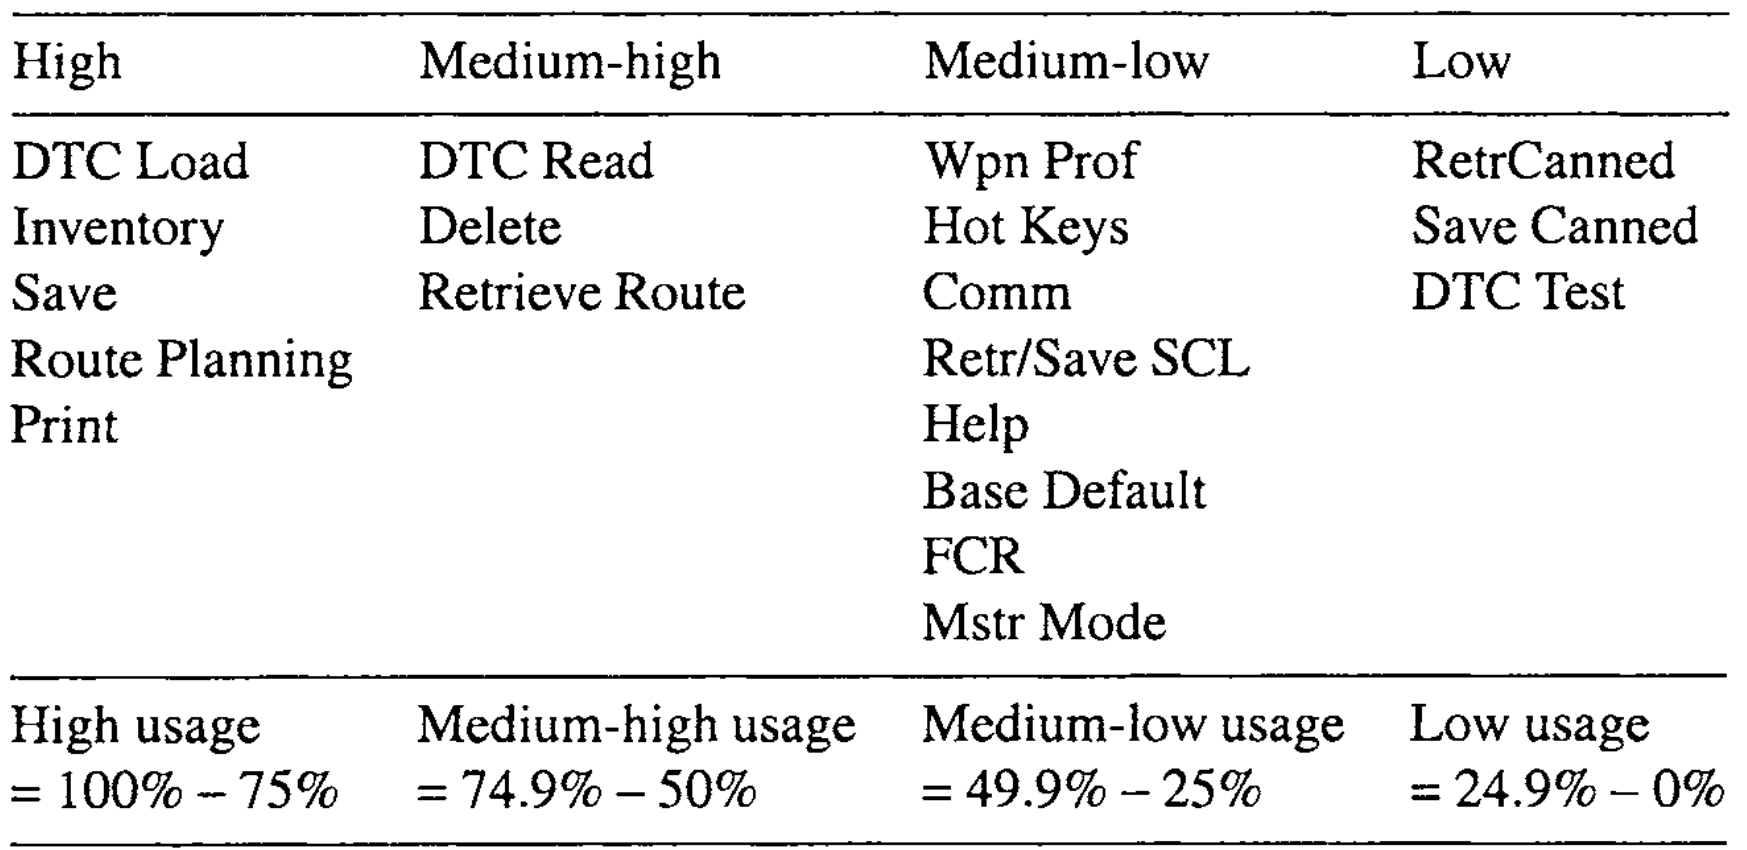
\includegraphics[width=\textwidth,height=0.7\textheight,keepaspectratio]{figure/CSSfunctions.png}
\end{center}
\end{frame}
%%%%%%%%%%%%%%%%%%%%%%%%%%%%%%%%%%%%%%%%%%%%%%%%%%%%%%%%%%%%%%%%%%%%%%%%
\subsection{8.5 メトリック収集, 結果検証, 経験}
\begin{frame}{メトリックを収集(p124)}
\framesubtitle{Metrics collections}
\begin{enumerate}
\item SPMに製品の市場を把握する
    \begin{itemize}
    \item 何週間に短いインタビュー
    \end{itemize}
\item SPMと議論し、ユーザープロフィールと機能プロフィールの要求を定義
    \begin{itemize}
    \item 既存のCSSの機能設計は役に立った
    \end{itemize}
\item System Engineers と Test Engineers の経験から、ユーザー調査書を作った
\item メールでのユーザー調査
\item 結果操作プロフィールの解釈
    \begin{itemize}
    \item 前の図と表で表す
    \end{itemize}
\end{enumerate}
\end{frame}

%%%%%%%%%%%%%%%%%%%%%%%%%%%%%%%%%%%%%%%%%%%%%%%%%%%%%%%%%%%%%%%%%%%%%%%%
\begin{frame}{結果を検証(p125)}
\framesubtitle{Result Validation}
意外の結果を解釈中に出た
\begin{itemize}
\item ホットキーの使用はMedium-low
    \begin{itemize}
    \item ユーザーは既存のホットキーを依存
    \end{itemize}
\item ヘルプ機能はMedium-low
    \begin{itemize}
    \item ユーザーはシステムにもっと詳しいと思った
    \end{itemize}
\end{itemize}
\end{frame}
%%%%%%%%%%%%%%%%%%%%%%%%%%%%%%%%%%%%%%%%%%%%%%%%%%%%%%%%%%%%%%%%%%%%%%%%
\section{8.6 まどめ}
\subsection{8.6 まどめ}
\begin{frame}{まどめ(p125)}
\framesubtitle{Concluding Remarks}
\begin{enumerate}
\item チェックリスト・テスト, とそれの制限を紹介した
\item 分割に基づくテストモデルを紹介した
    \begin{itemize}
    \item 9章に入力ドメインによる分割と境界テストを紹介する
    \end{itemize}
\item Musaによる操作プロフィール(OP)を紹介した
    \begin{itemize}
    \item Musa-1 多数OP
    \item Musa-2 単一OP
    \item CSSの事例
    \end{itemize}
\end{enumerate}
もっと複雑のプログラムに使うFSMに基づくモデルを10, 11章に紹介する
\end{frame}

%%%%%%%%%%%%%%%%%%%%%%%%%%%%%%%%%%%%%%%%%%%%%%%%%%%%%%%%%%%%%%%%%%%%%%%%
\appendix
\backupbegin
\begin{frame}{Reference}

\bibliographystyle{IEEEtranN}
\bibliography{chapter8}
\end{frame}
\backupend
\end{document}
